% -------------------------------------------------
% Anexo C. Interfaces del módulo Aprender a Aprender
% -------------------------------------------------
\section*{Anexo C. Interfaces del módulo Aprender a Aprender}
\addcontentsline{toc}{section}{Anexo C.  Interfaces del módulo Aprender a Aprender}
\label{anexo:interfaces_aprender}

Este anexo presenta las interfaces asociadas a cada una de las actividades descritas en la sección \textit{“Actividades implementadas en el módulo aprender a aprender”}. Las figuras se organizan en el mismo orden en que aparecen las actividades, con el fin de facilitar la vinculación entre la descripción funcional y su implementación visual dentro del prototipo.

% -------------------------------------------------
\subsection*{Creación de roadmaps personalizados}
% -------------------------------------------------

\begin{figure}[H]
\centering
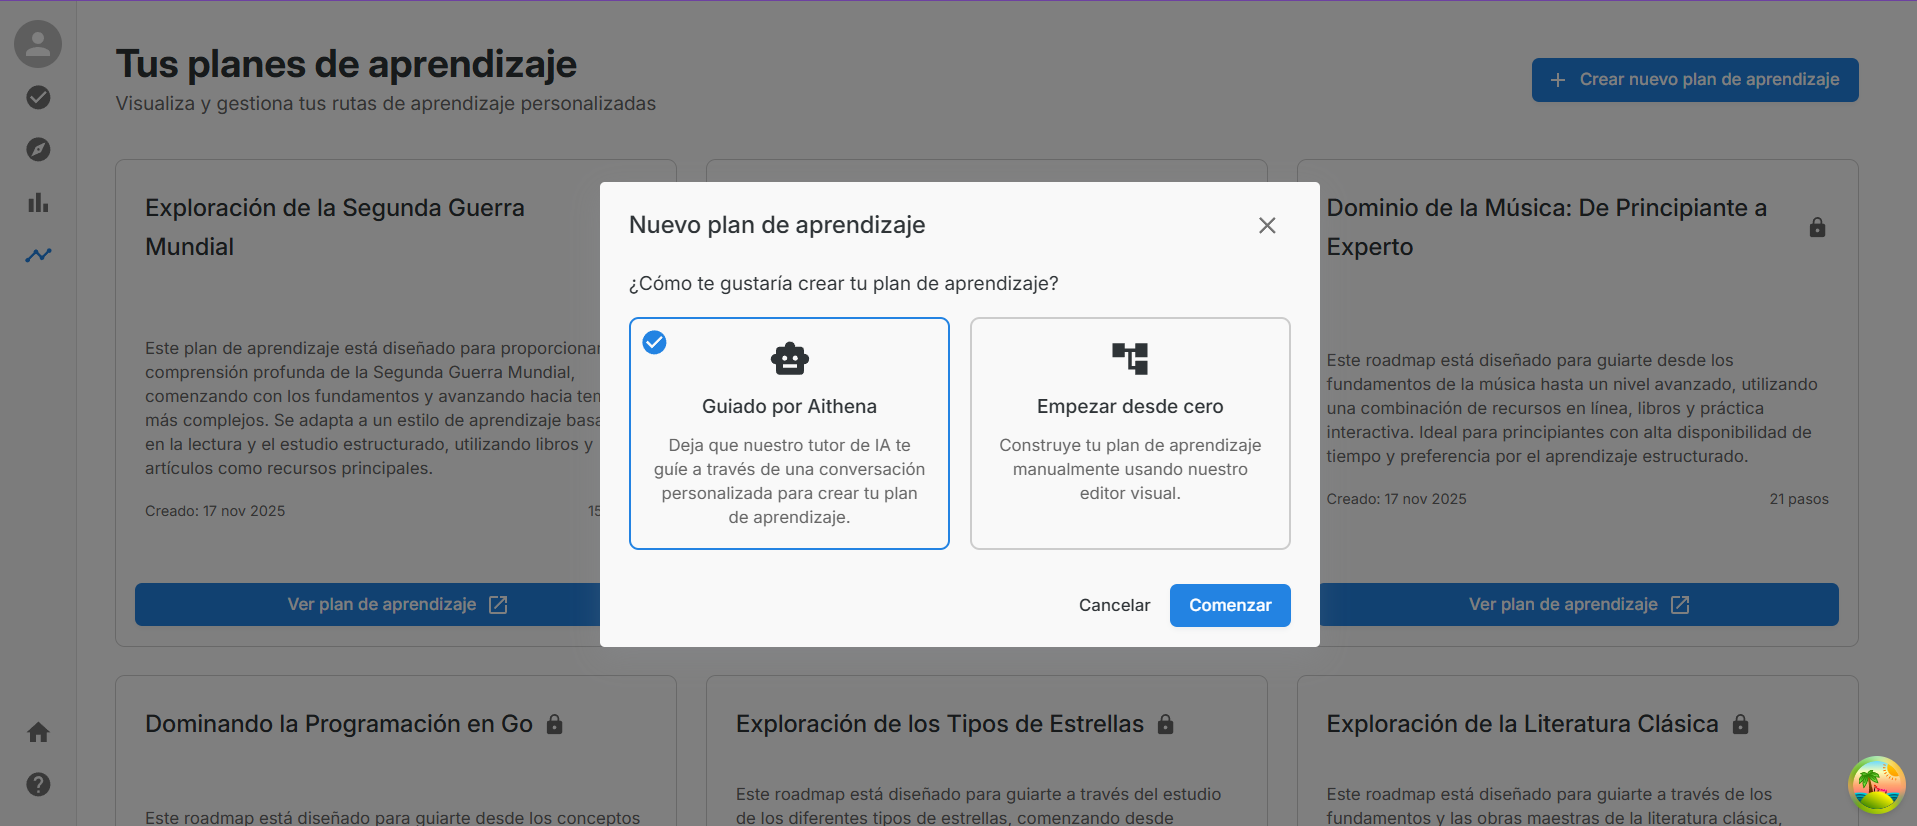
\includegraphics[width=0.95\textwidth]{Figuras/interfaces_AaA/creacion_roadmap.png}
\caption{Interfaz para la creación de roadmaps personalizados.}
\label{fig:aprender-creacion-roadmap}
\end{figure}

\noindent\textit{Descripción.} La interfaz permite elegir entre generar un roadmap automático mediante un agente de inteligencia artificial, que propone una ruta de aprendizaje personalizada, o bien construir un roadmap manual desde cero a través del editor visual.
\\
\\

% -------------------------------------------------
\subsection*{Edición mediante un editor visual de planes de aprendizaje}
% -------------------------------------------------

\noindent\textit{Descripción.} El editor permite añadir objetivos, crear tareas, reorganizar elementos mediante arrastrar y soltar, modificar descripciones y visualizar la relación jerárquica entre los componentes del roadmap. En las Figuras~\ref{fig:editor-inicial} a~\ref{fig:editor-estructura-general} se ilustran estas acciones dentro de la interfaz.

% (1) Editor vacío: lienzo y componentes
\begin{figure}[H]
\centering
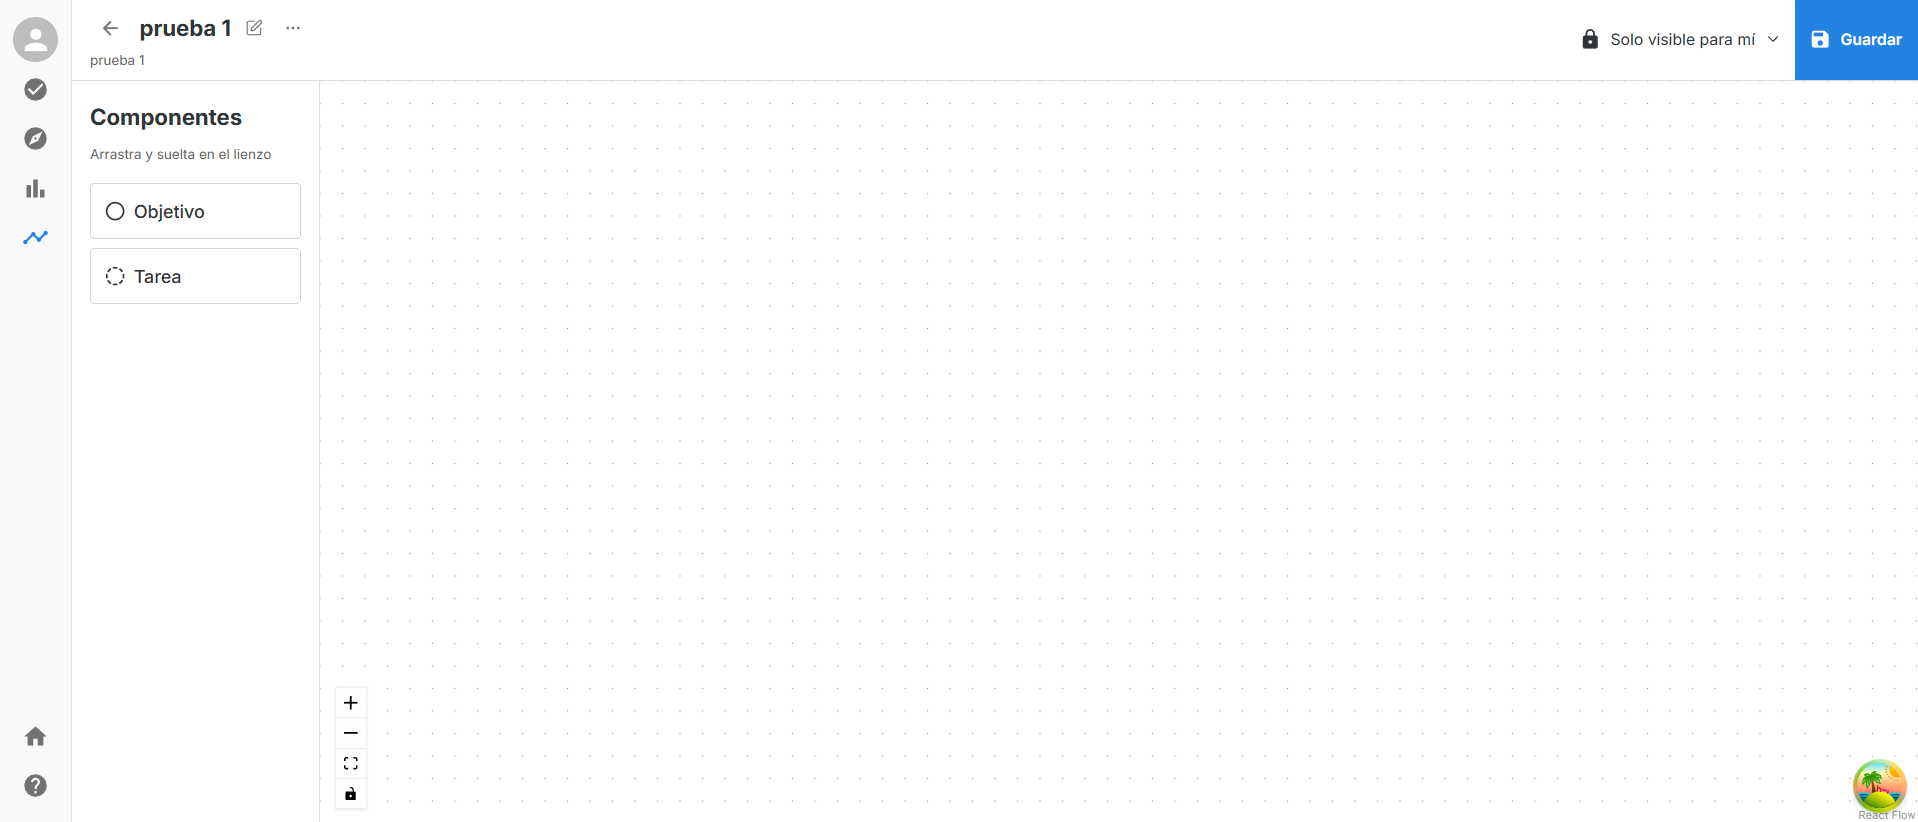
\includegraphics[width=0.95\textwidth]{Figuras/interfaces_AaA/editor_inicial.png}
\caption{Vista inicial del editor visual de planes de aprendizaje, con el lienzo y los componentes disponibles.}
\label{fig:editor-inicial}
\end{figure}

% (2) Arrastrar objetivo al lienzo
\begin{figure}[H]
\centering
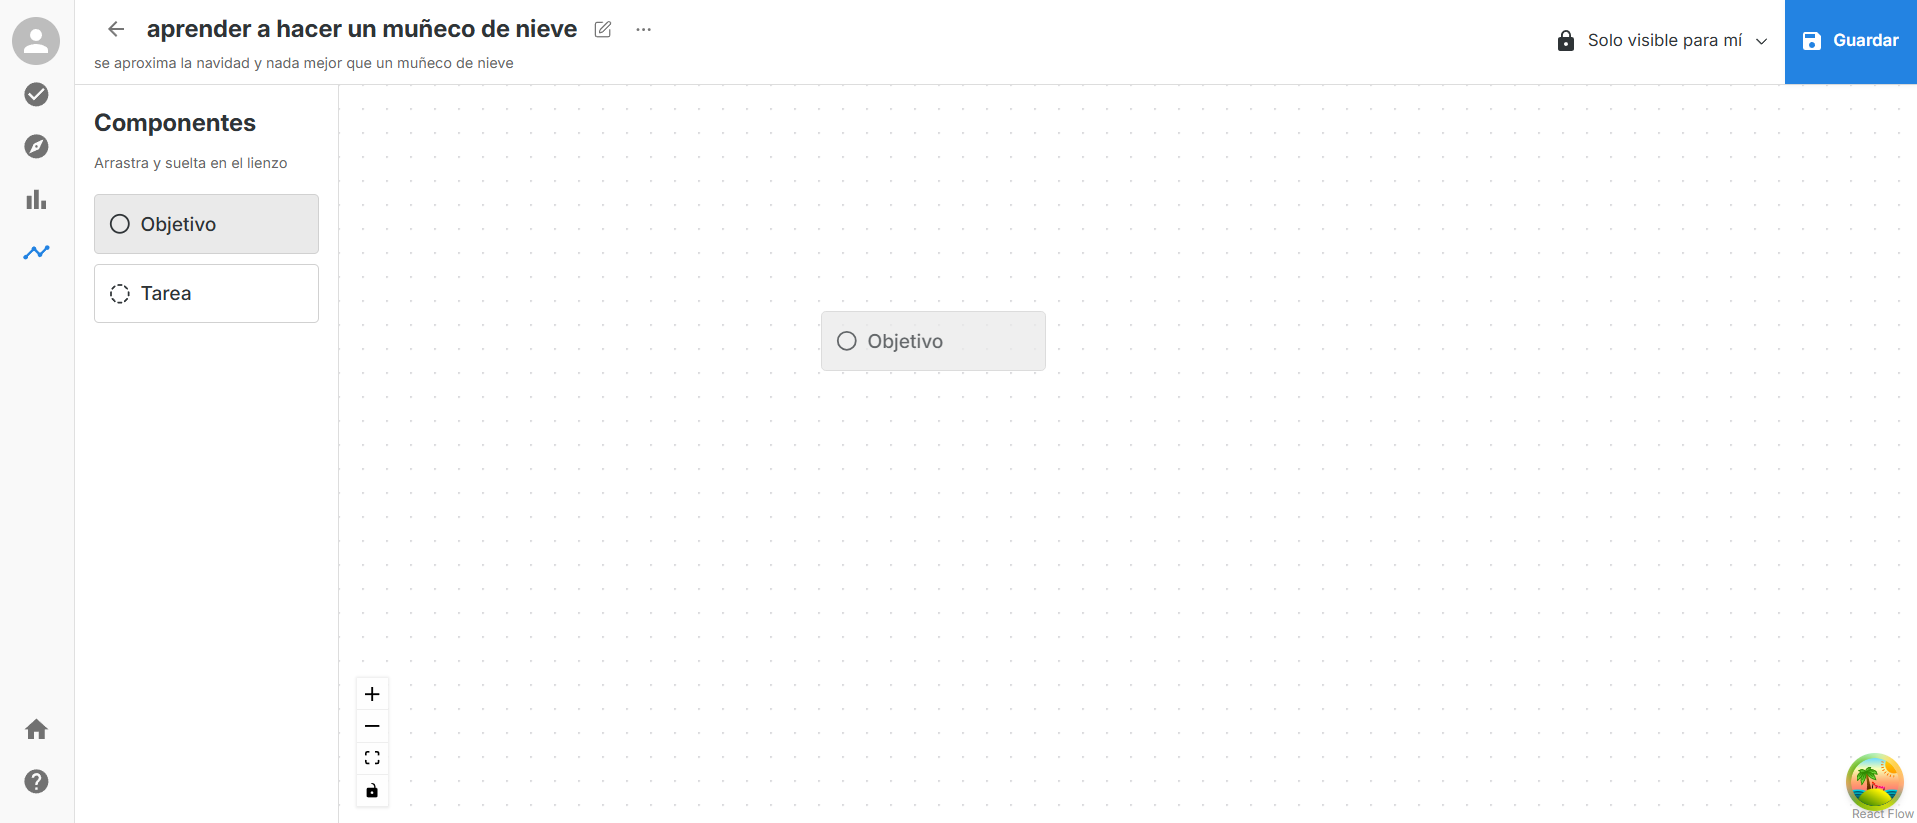
\includegraphics[width=0.95\textwidth]{Figuras/interfaces_AaA/editor_agregar_objetivo.png}
\caption{Agregar un nuevo objetivo arrastrándolo desde el panel de componentes hacia el lienzo.}
\label{fig:editor-agregar-objetivo}
\end{figure}

% (3) Arrastrar tarea al lienzo
\begin{figure}[H]
\centering
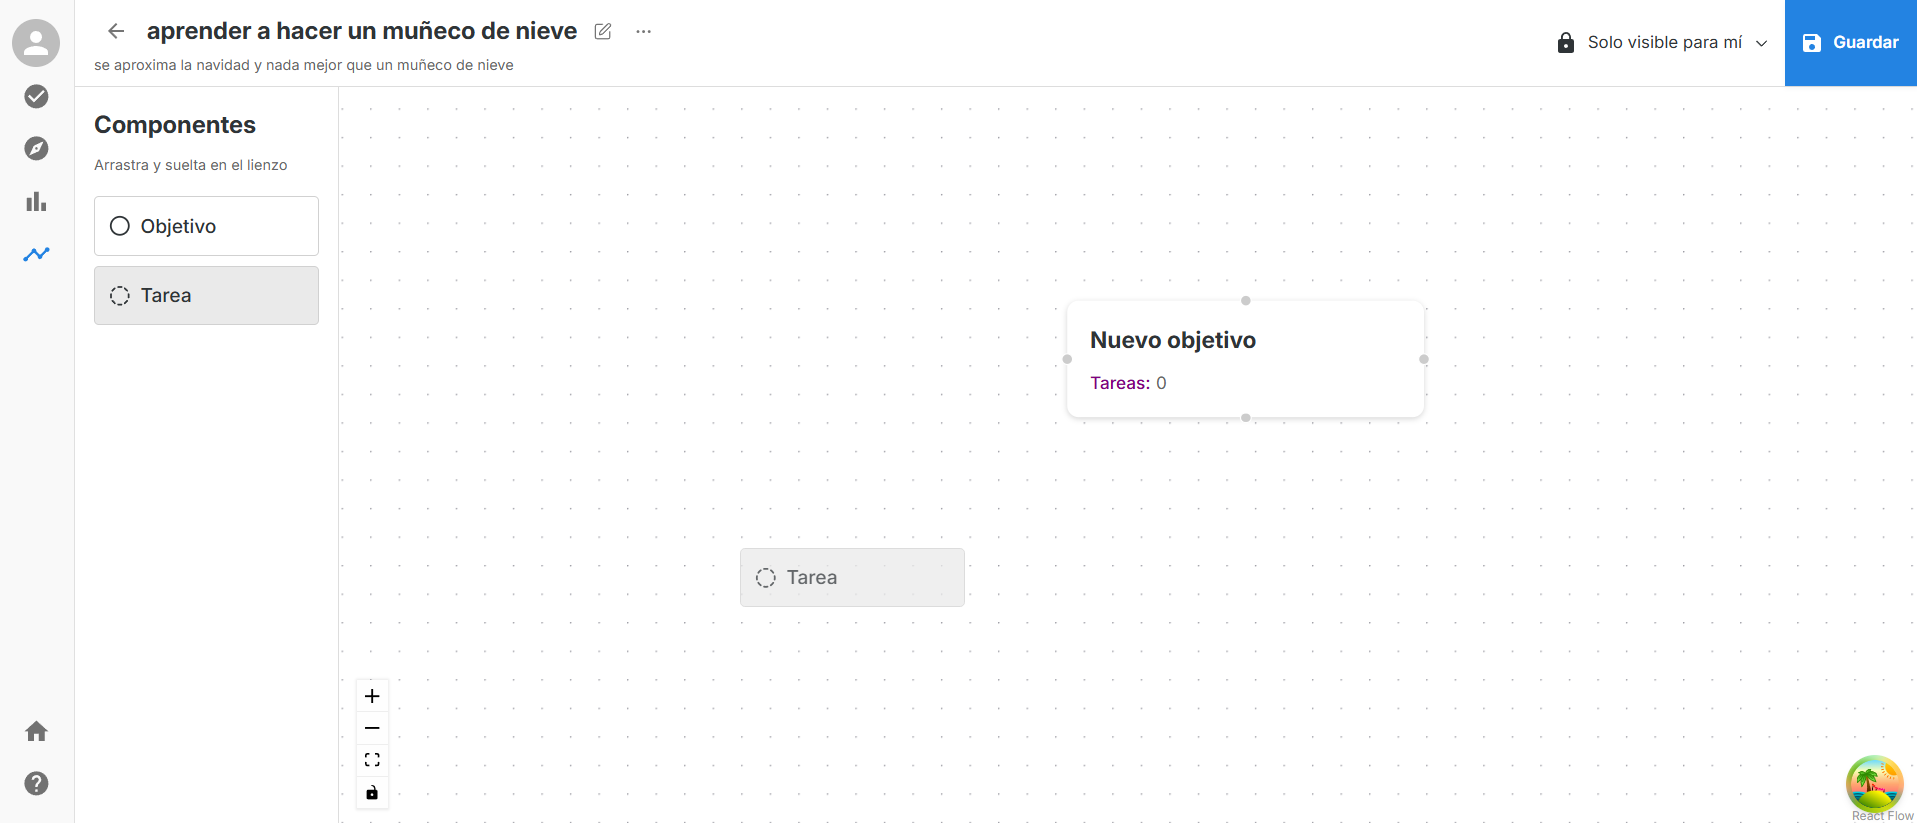
\includegraphics[width=0.95\textwidth]{Figuras/interfaces_AaA/editor_agregar_tarea.png}
\caption{Agregar una tarea al plan de aprendizaje mediante arrastrar y soltar.}
\label{fig:editor-agregar-tarea}
\end{figure}

% (4) Conectar tarea con objetivo
\begin{figure}[H]
\centering
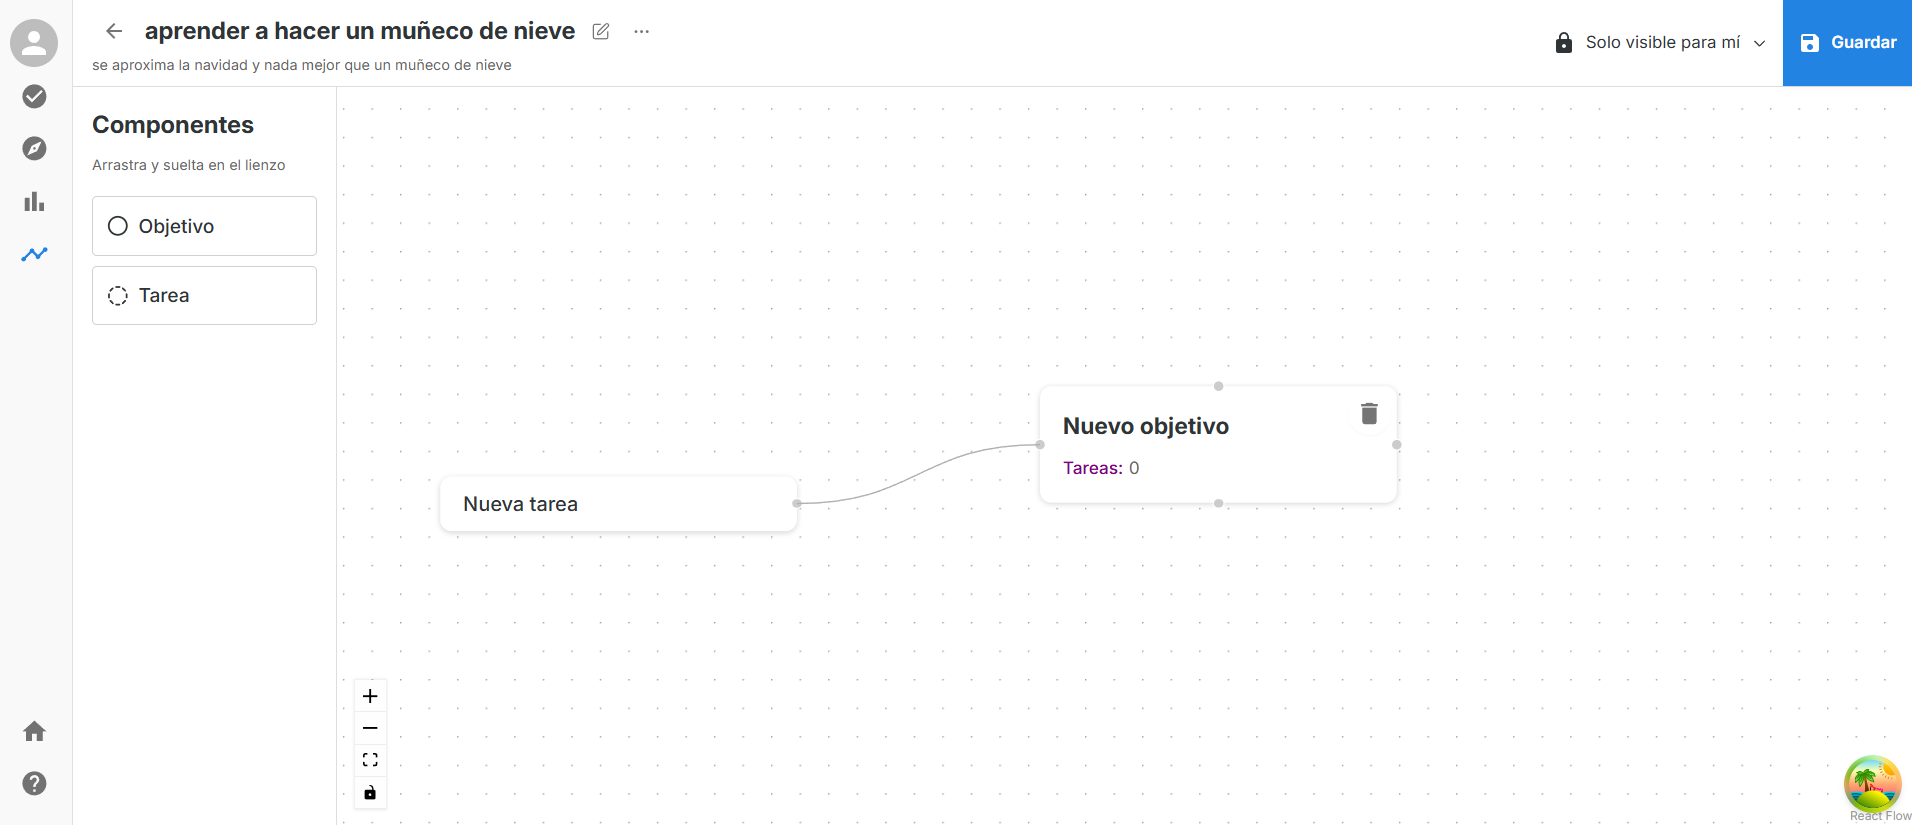
\includegraphics[width=0.95\textwidth]{Figuras/interfaces_AaA/editor_conectar_tarea_a_objetivo.png}
\caption{Conexión de una tarea con un objetivo, representando la relación entre ambos componentes.}
\label{fig:editor-conectar-tarea}
\end{figure}

% (5) Edición de contenido y enlaces del nodo
\begin{figure}[H]
\centering
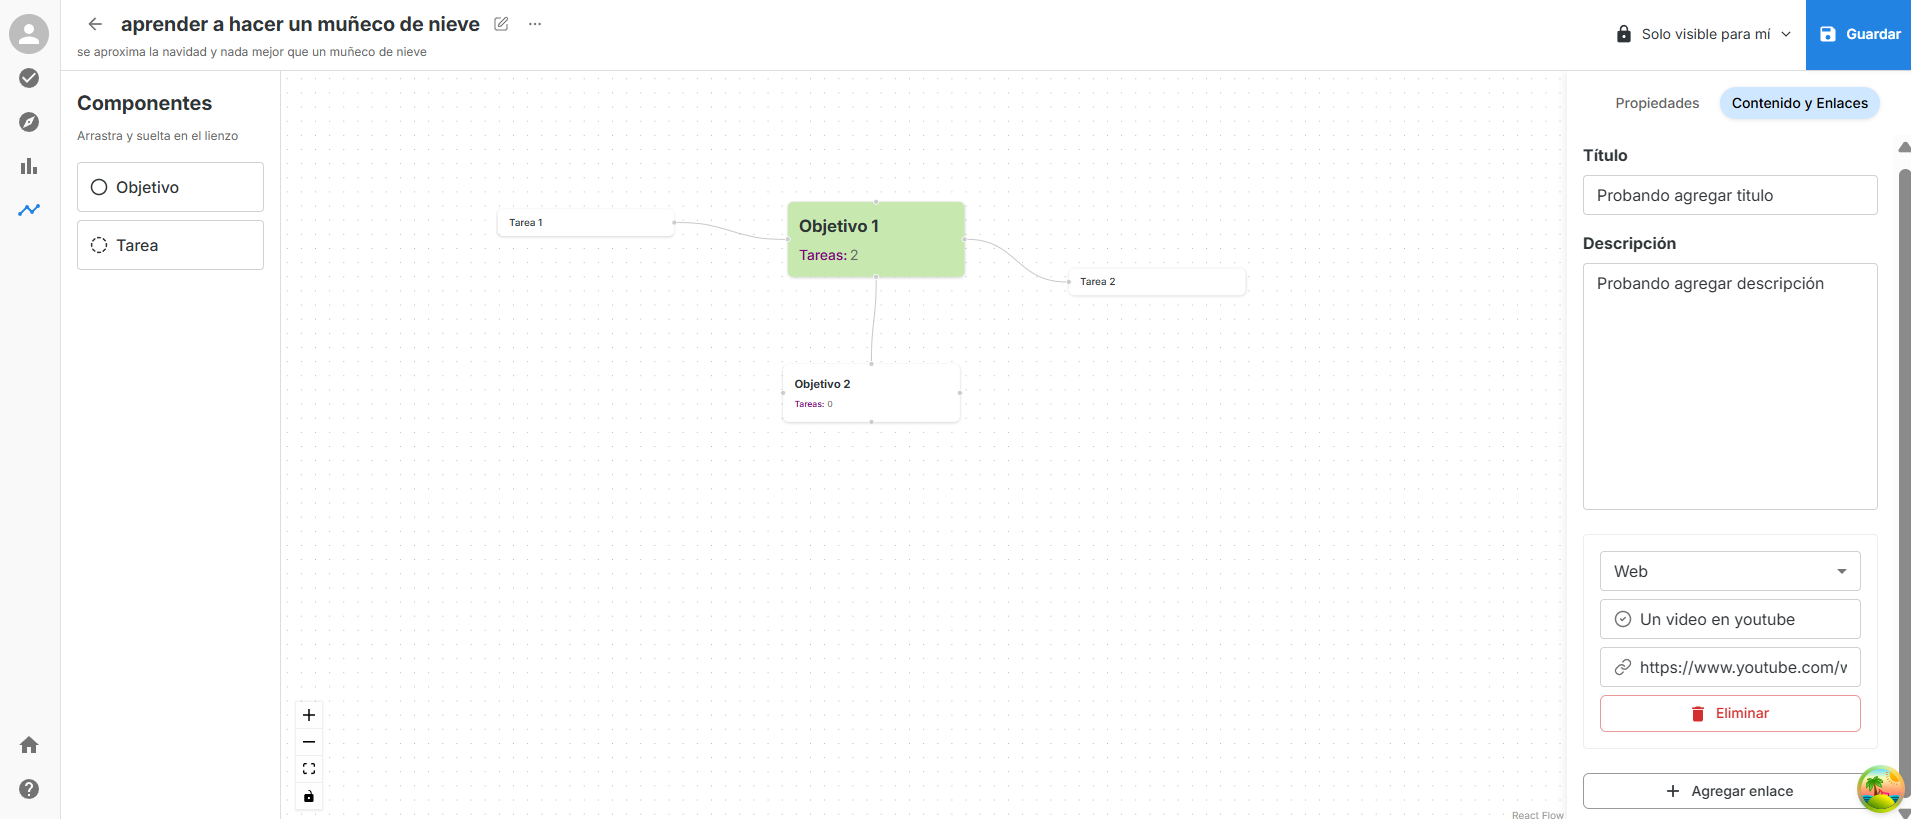
\includegraphics[width=0.95\textwidth]{Figuras/interfaces_AaA/editor_editar_contenido_y_enlaces.png}
\caption{Edición del contenido del objetivo y gestión de recursos asociados desde el panel lateral.}
\label{fig:editor-contenido-enlaces}
\end{figure}

% (6) Edición de propiedades visuales del nodo
\begin{figure}[H]
\centering
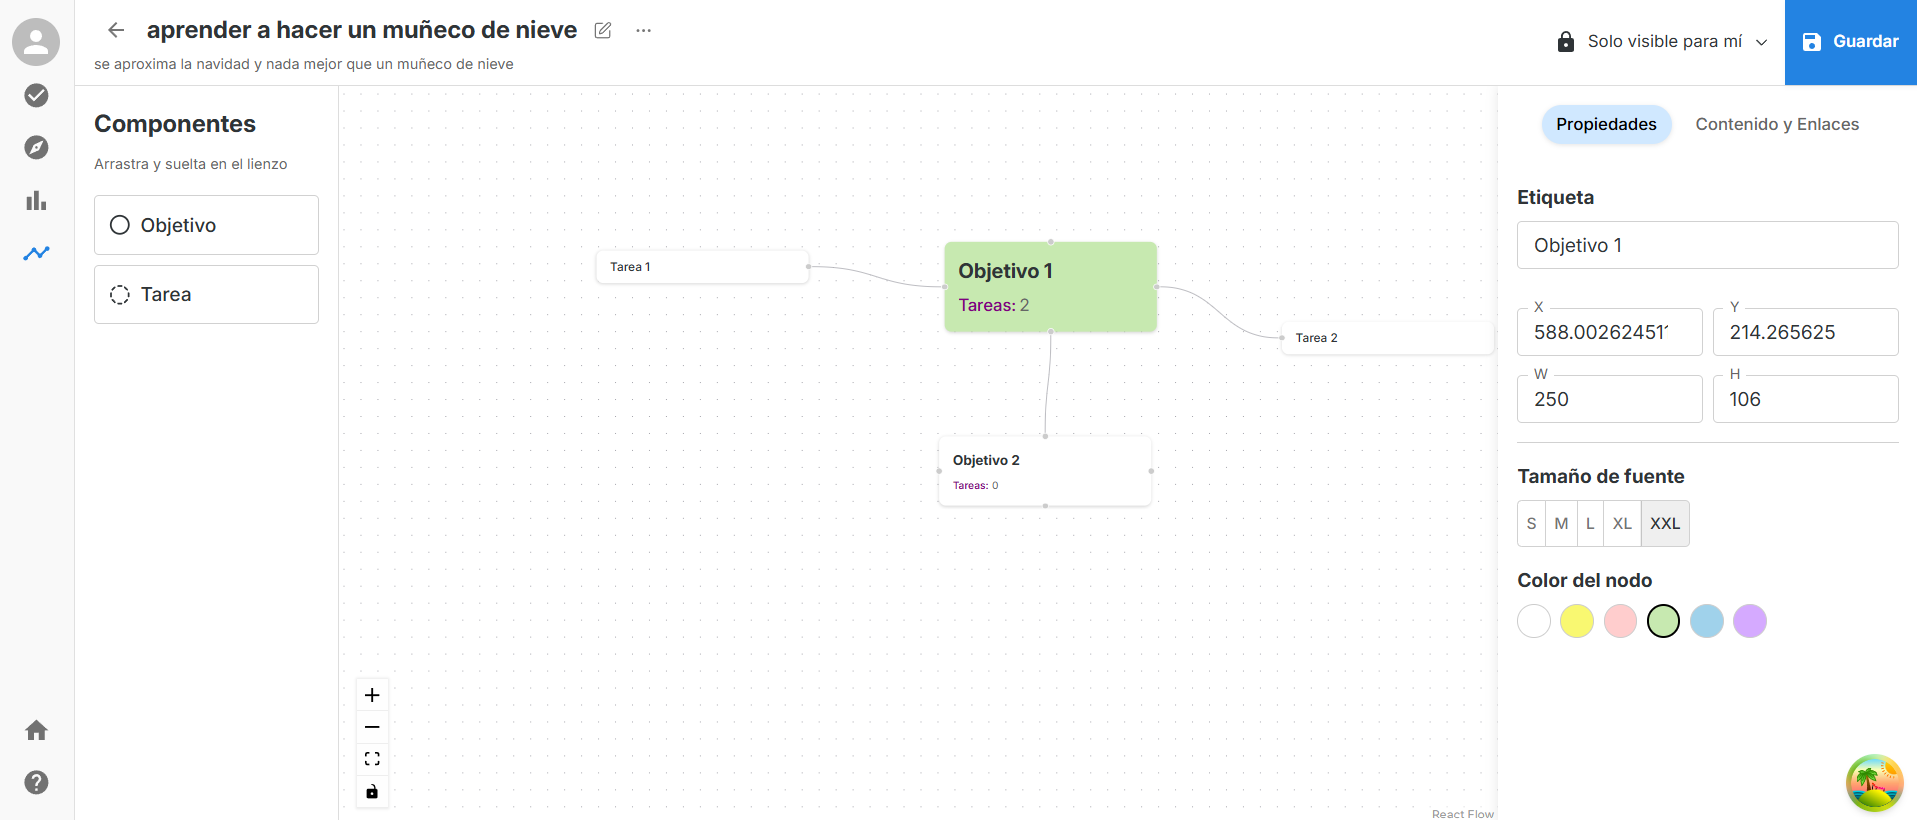
\includegraphics[width=0.95\textwidth]{Figuras/interfaces_AaA/editor_editar_propiedades_nodo.png}
\caption{Configuración de las propiedades visuales del objetivo (posición, tamaño y color del nodo).}
\label{fig:editor-propiedades-nodo}
\end{figure}

% (7) Estructura general del roadmap
\begin{figure}[H]
\centering
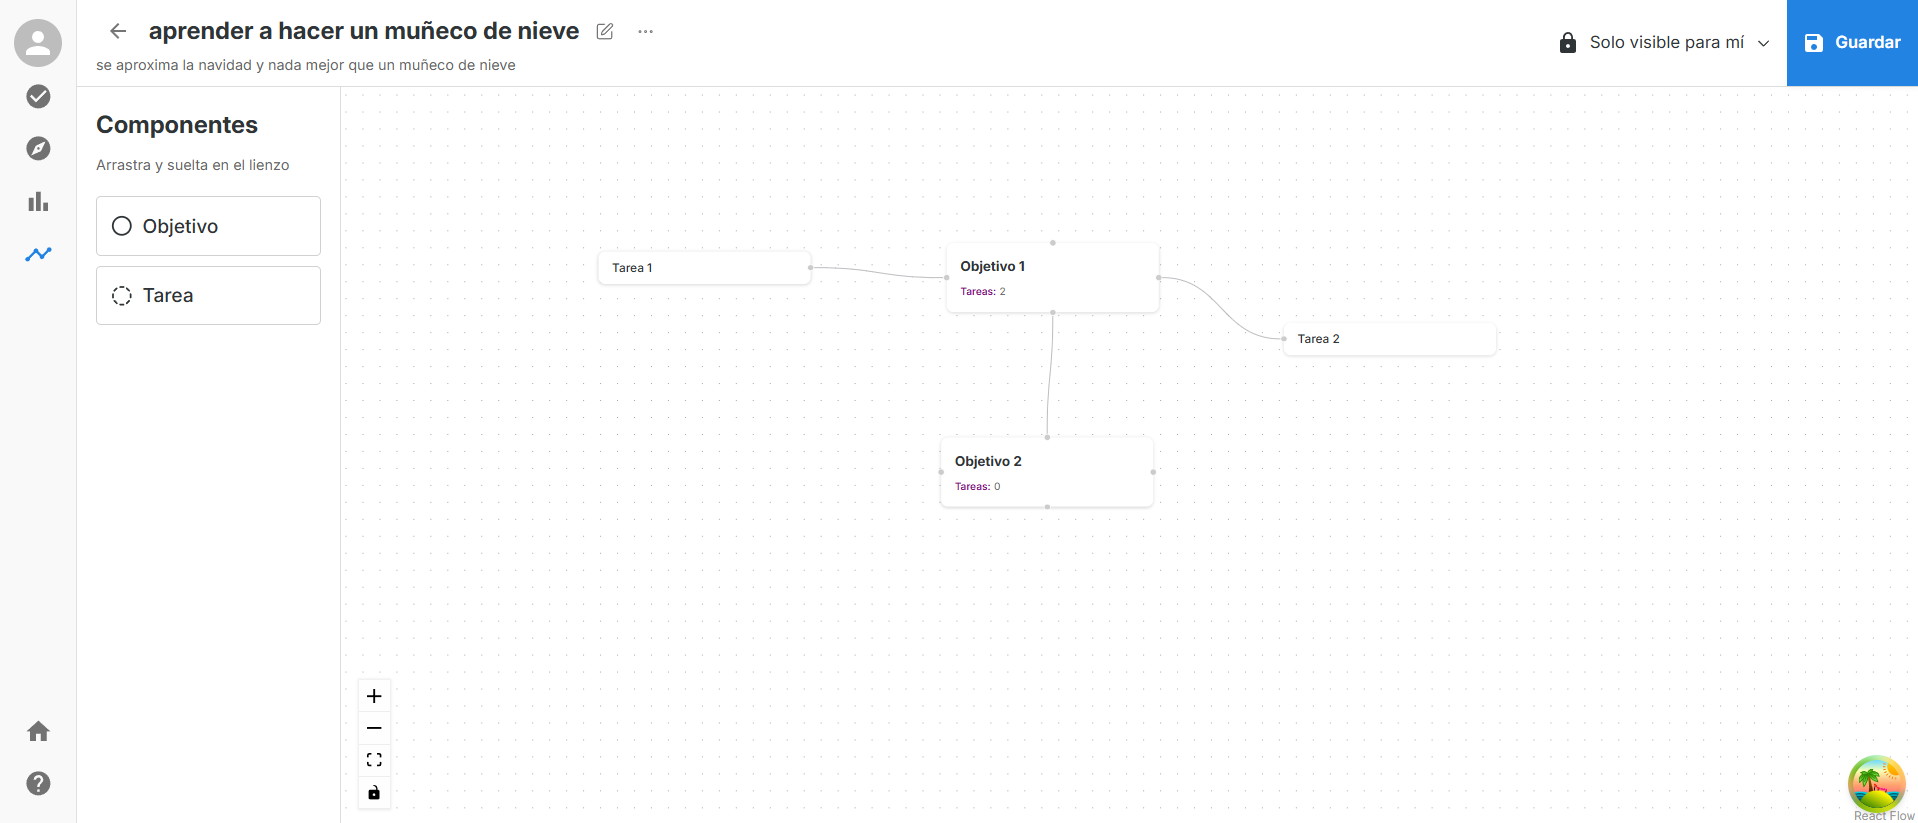
\includegraphics[width=0.95\textwidth]{Figuras/interfaces_AaA/editor_estructura_general.png}
\caption{Vista de la estructura general del roadmap, mostrando la relación jerárquica entre objetivos y tareas.}
\label{fig:editor-estructura-general}
\end{figure}

% -------------------------------------------------
\subsection*{Conversión entre roadmap y plan accionable}
% -------------------------------------------------

% (1) Opción: Crear plan accionable desde un roadmap
\begin{figure}[H]
\centering
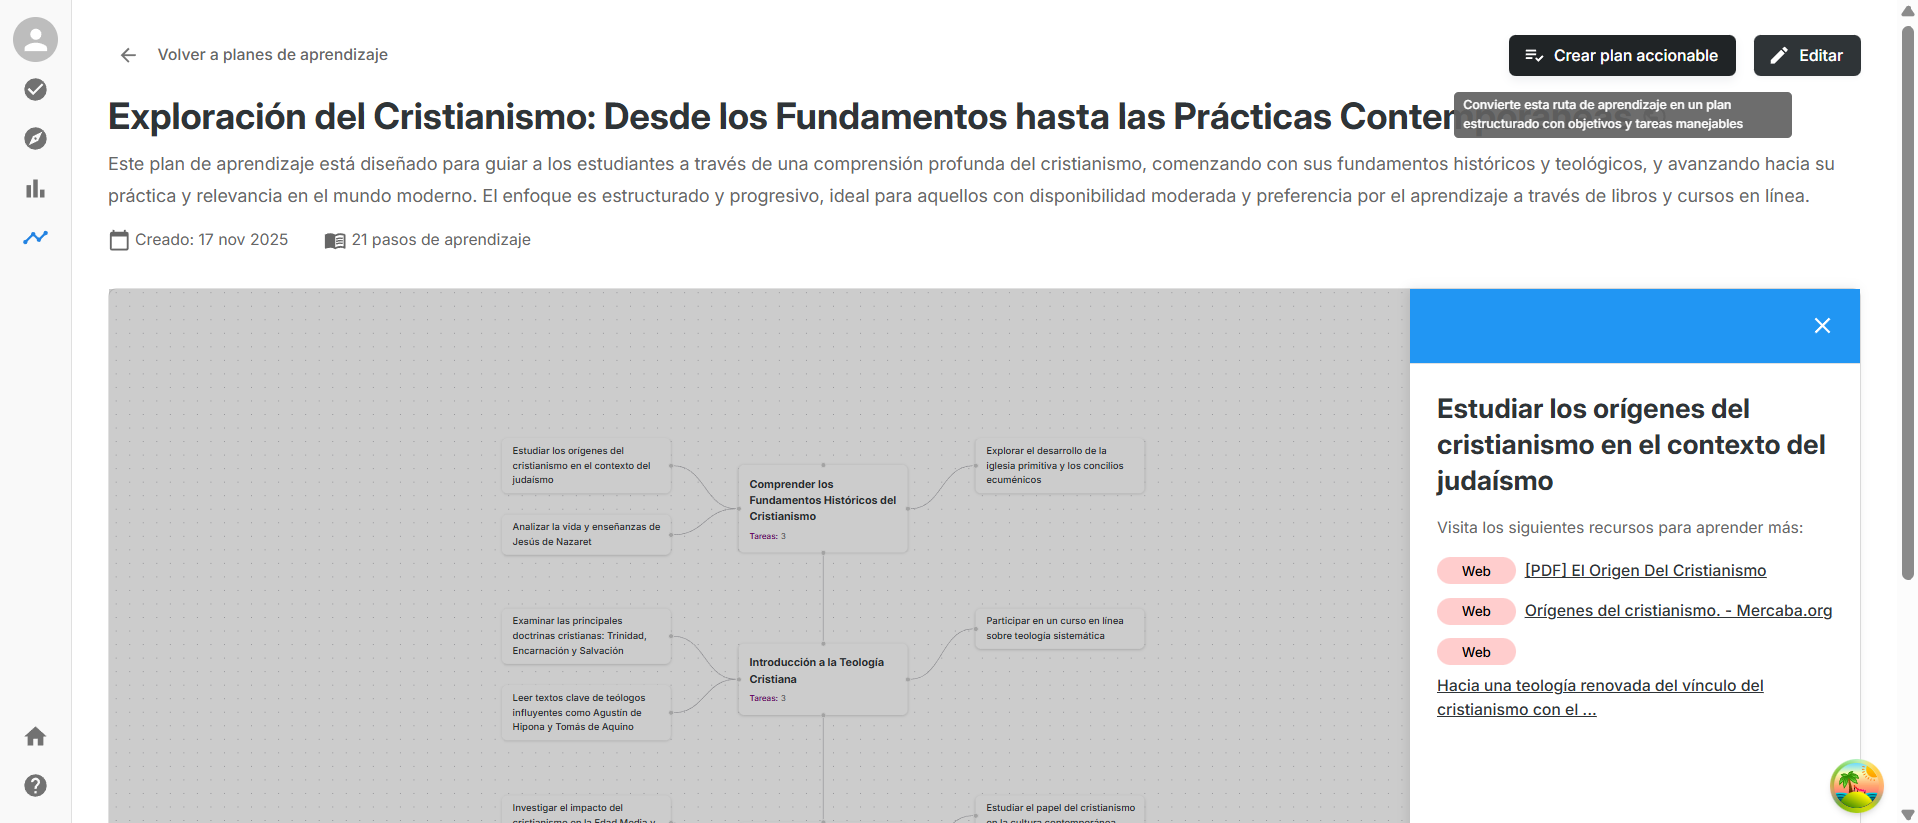
\includegraphics[width=0.95\textwidth]{Figuras/interfaces_AaA/roadmap_crear_plan_accionable.png}
\caption{Opción disponible en la vista del roadmap para crear un plan accionable a partir de la estructura diseñada.}
\label{fig:crear-plan-accionable}
\end{figure}

\noindent\textit{Descripción.} Desde la vista del roadmap, el estudiante puede convertir la ruta de aprendizaje en un plan accionable con un solo clic. Esta función genera automáticamente la meta principal, los objetivos y las tareas basadas en el contenido del roadmap, manteniendo su organización jerárquica.

% (2) Transformar plan accionable a roadmap
\begin{figure}[H]
\centering
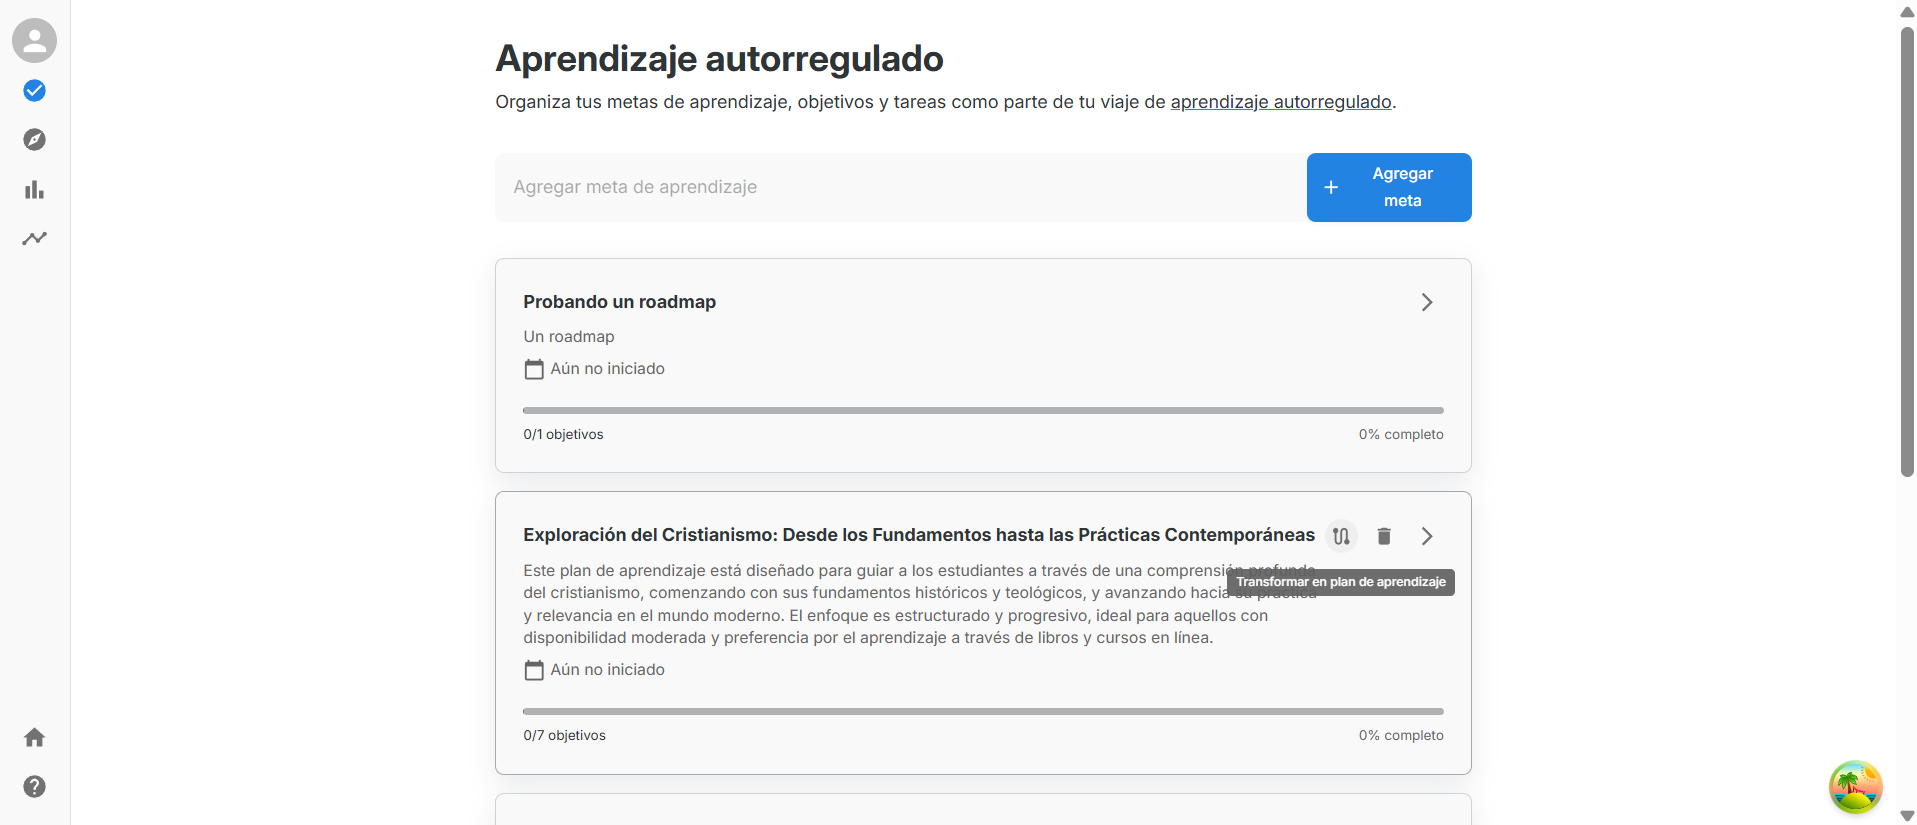
\includegraphics[width=0.95\textwidth]{Figuras/interfaces_AaA/plan_accionable_transformar_a_roadmap.png}
\caption{Interfaz que permite transformar un plan accionable existente nuevamente en un roadmap visual.}
\label{fig:accionable-a-roadmap}
\end{figure}

\noindent\textit{Descripción.} La conversión inversa permite visualizar un plan estructurado como un roadmap, facilitando la comprensión global de su organización y permitiendo reorganizar la estructura mediante el editor visual.


% (3) Lista de metas del plan accionable
\begin{figure}[H]
\centering
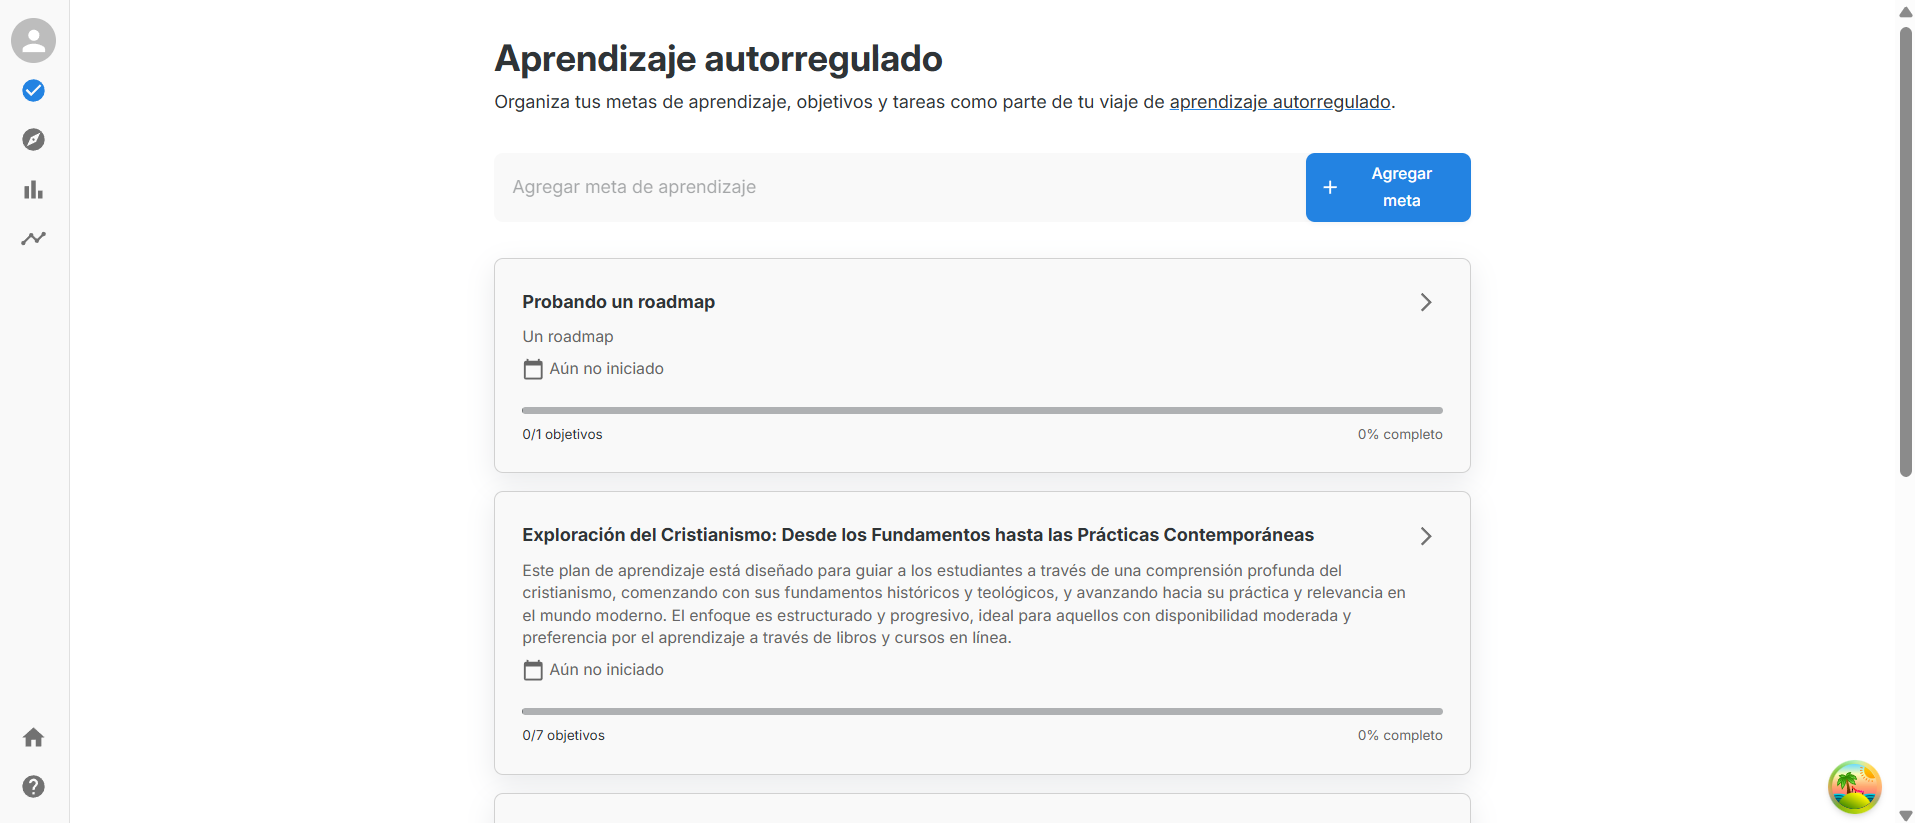
\includegraphics[width=0.95\textwidth]{Figuras/interfaces_AaA/plan_accionable_lista_metas.png}
\caption{Vista general del módulo de aprendizaje autorregulado, mostrando las metas generadas a partir del roadmap.}
\label{fig:accionable-lista-metas}
\end{figure}

\noindent\textit{Descripción.} Una vez generado el plan accionable, este aparece en la vista general del módulo, donde el estudiante puede acceder a su progreso, ver la cantidad de objetivos asociados y gestionar el avance en cada uno de ellos.

% (4) Detalle de una meta convertida
\begin{figure}[H]
\centering
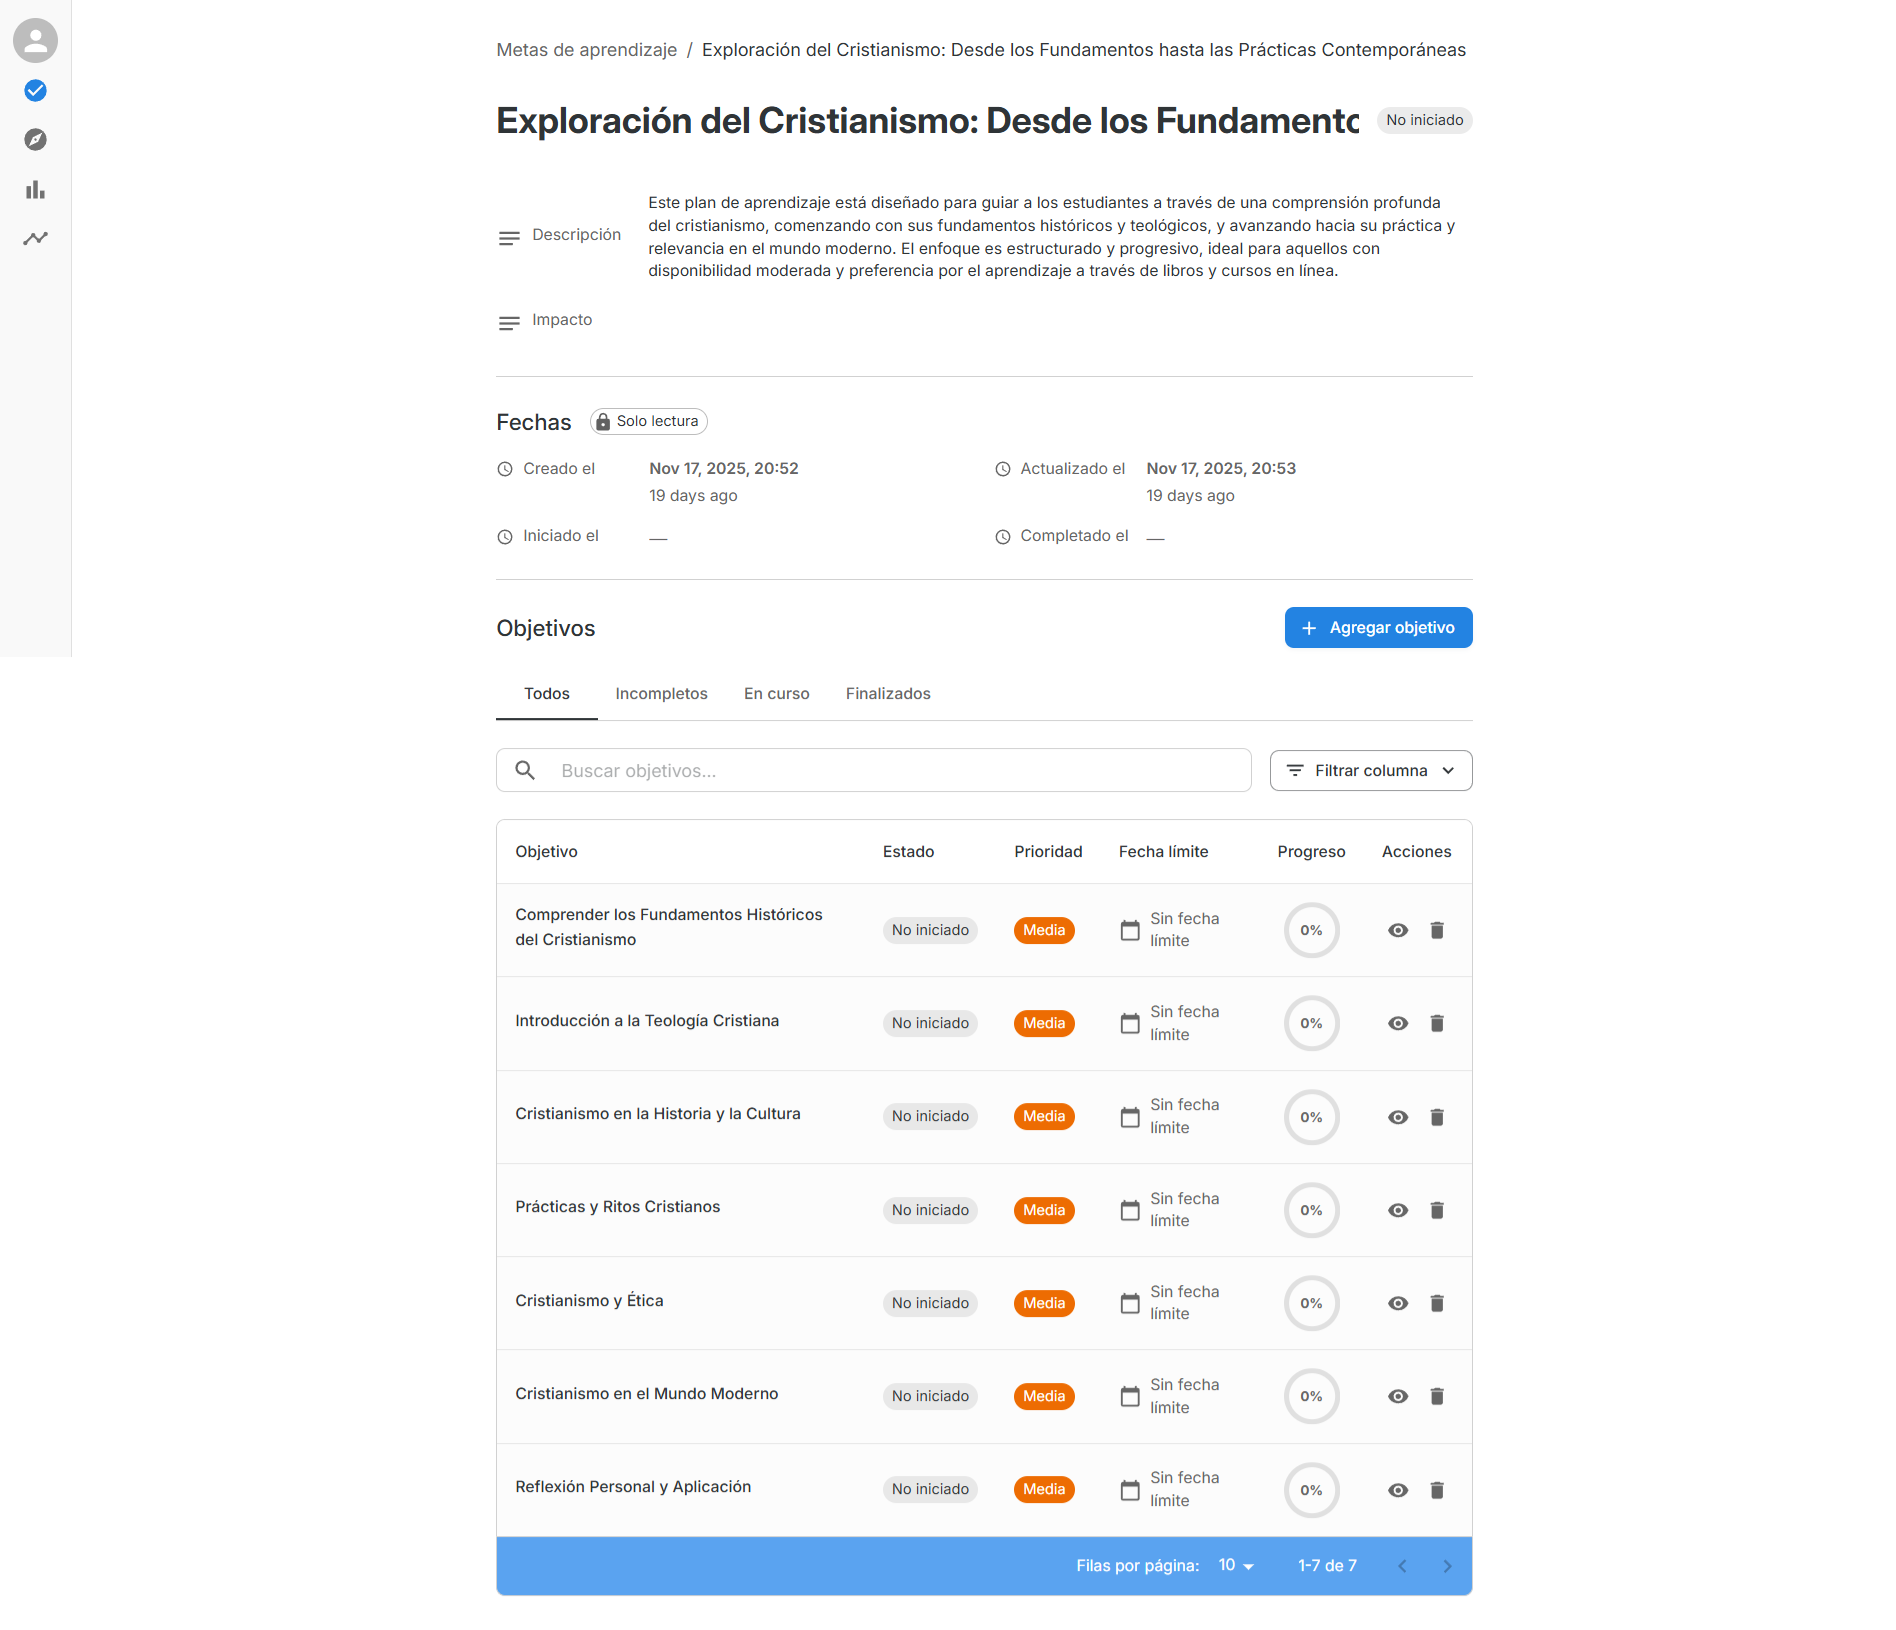
\includegraphics[width=0.95\textwidth]{Figuras/interfaces_AaA/plan_accionable_detalle_meta.png}
\caption{Vista detallada de la meta generada desde el roadmap, mostrando la lista completa de objetivos asociados.}
\label{fig:accionable-detalle-meta}
\end{figure}

\noindent\textit{Descripción.} La meta incluye todos los objetivos derivados del roadmap. Al convertirse en un plan accionable, cada objetivo se inicializa con una prioridad media y un estado por defecto, permitiendo al estudiante navegar entre ellos y revisar su contenido dentro de la estructura operativa del plan.


% (5) Detalle de un objetivo dentro del plan accionable
\begin{figure}[H]
\centering
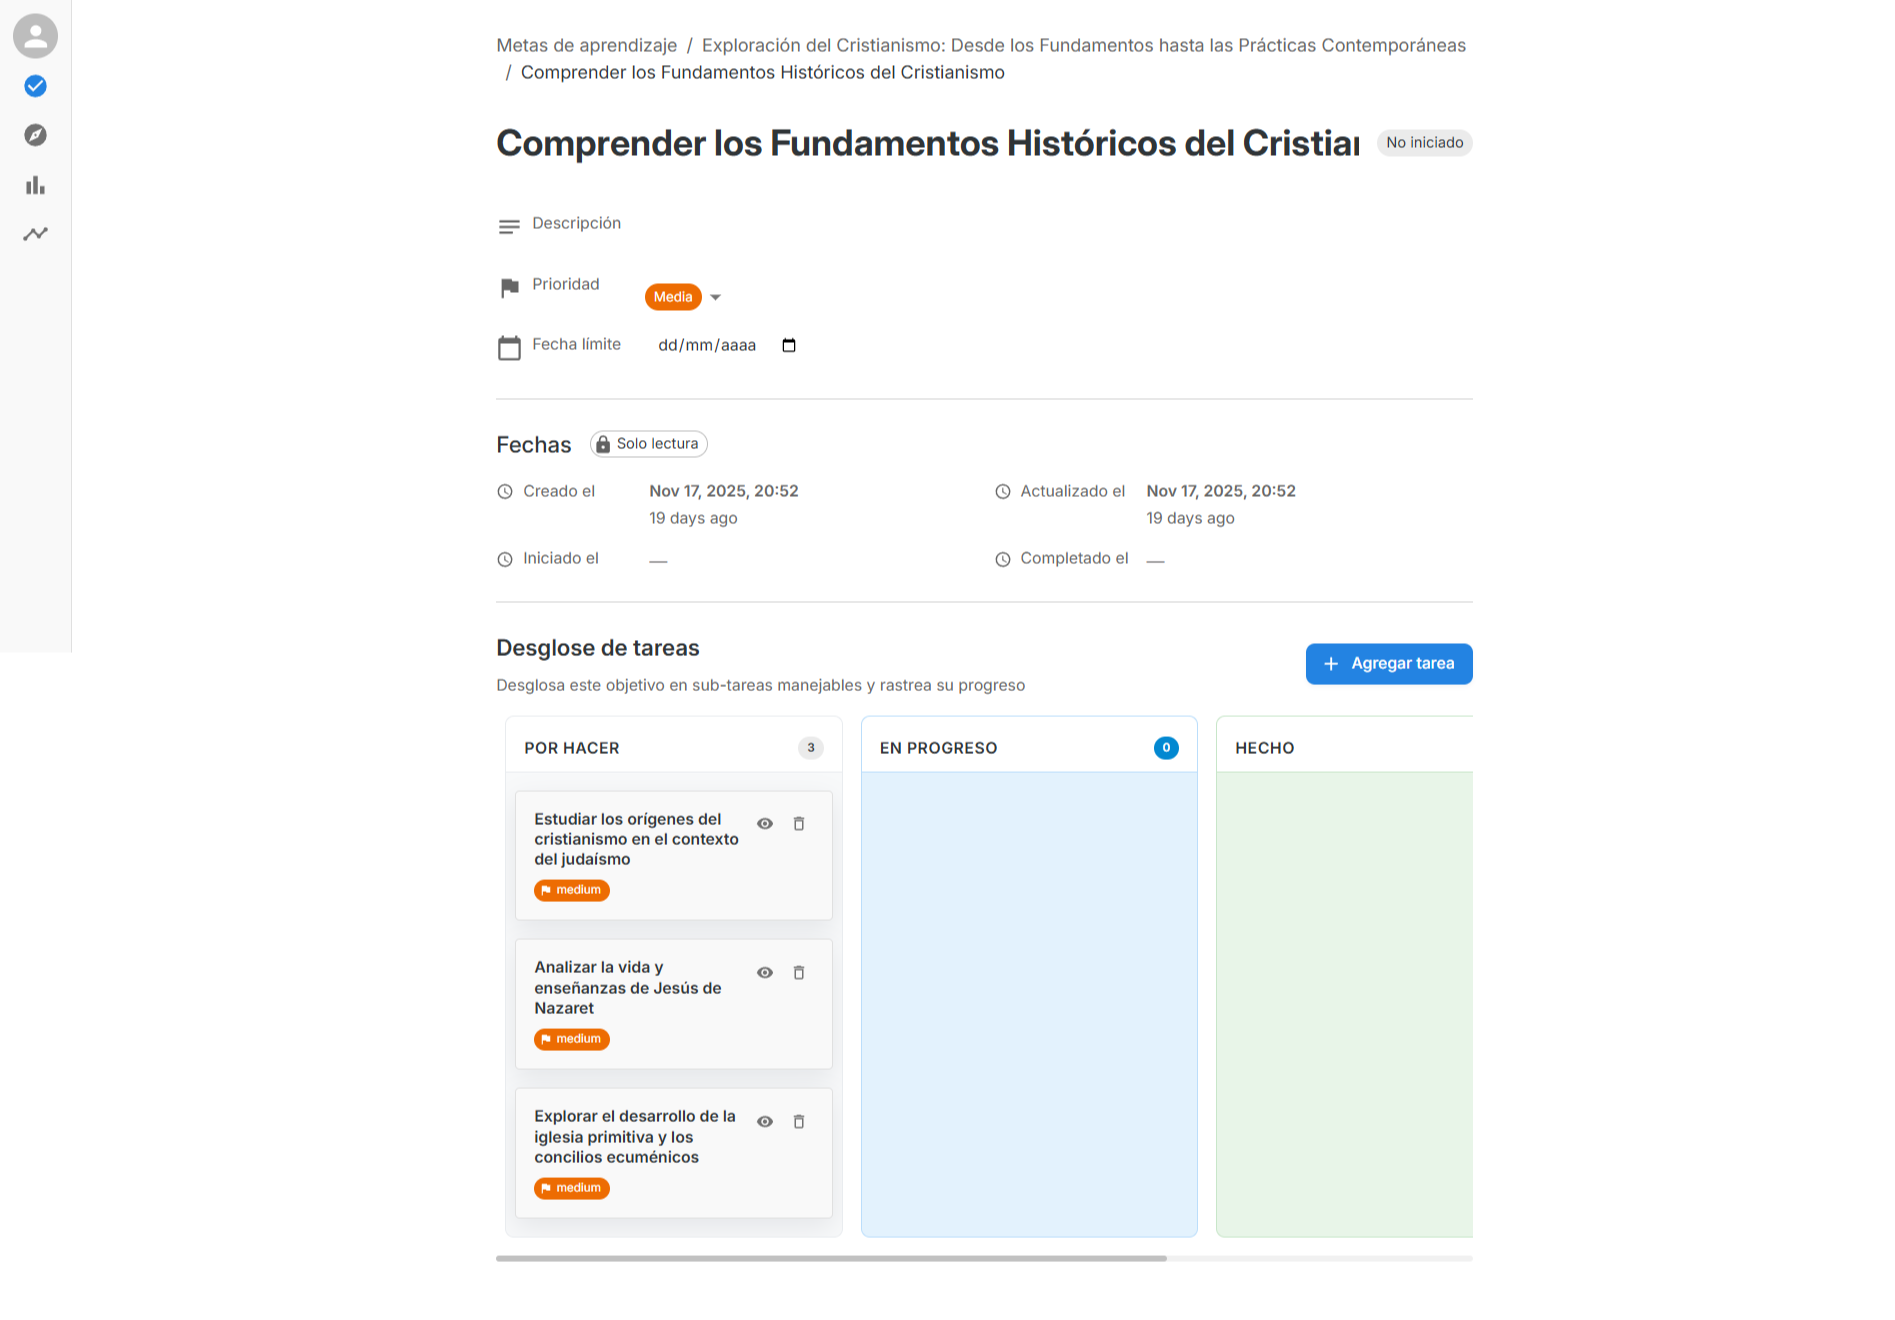
\includegraphics[width=0.95\textwidth]{Figuras/interfaces_AaA/plan_accionable_detalle_objetivo.png}
\caption{Interfaz de detalle de un objetivo dentro del plan accionable, con su desglose de tareas organizado por columnas de progreso.}
\label{fig:accionable-detalle-objetivo}
\end{figure}

\noindent\textit{Descripción.} Las tareas derivadas del roadmap se organizan automáticamente dentro del objetivo correspondiente y se presentan en columnas de \textit{Por hacer}, \textit{En progreso} y \textit{Hecho}. Al convertirse en plan accionable, cada tarea se inicializa con una prioridad media por defecto, manteniendo el título y la estructura definidos en el roadmap.



% (6) Detalle de una tarea convertida con recursos transferidos
\begin{figure}[H]
\centering
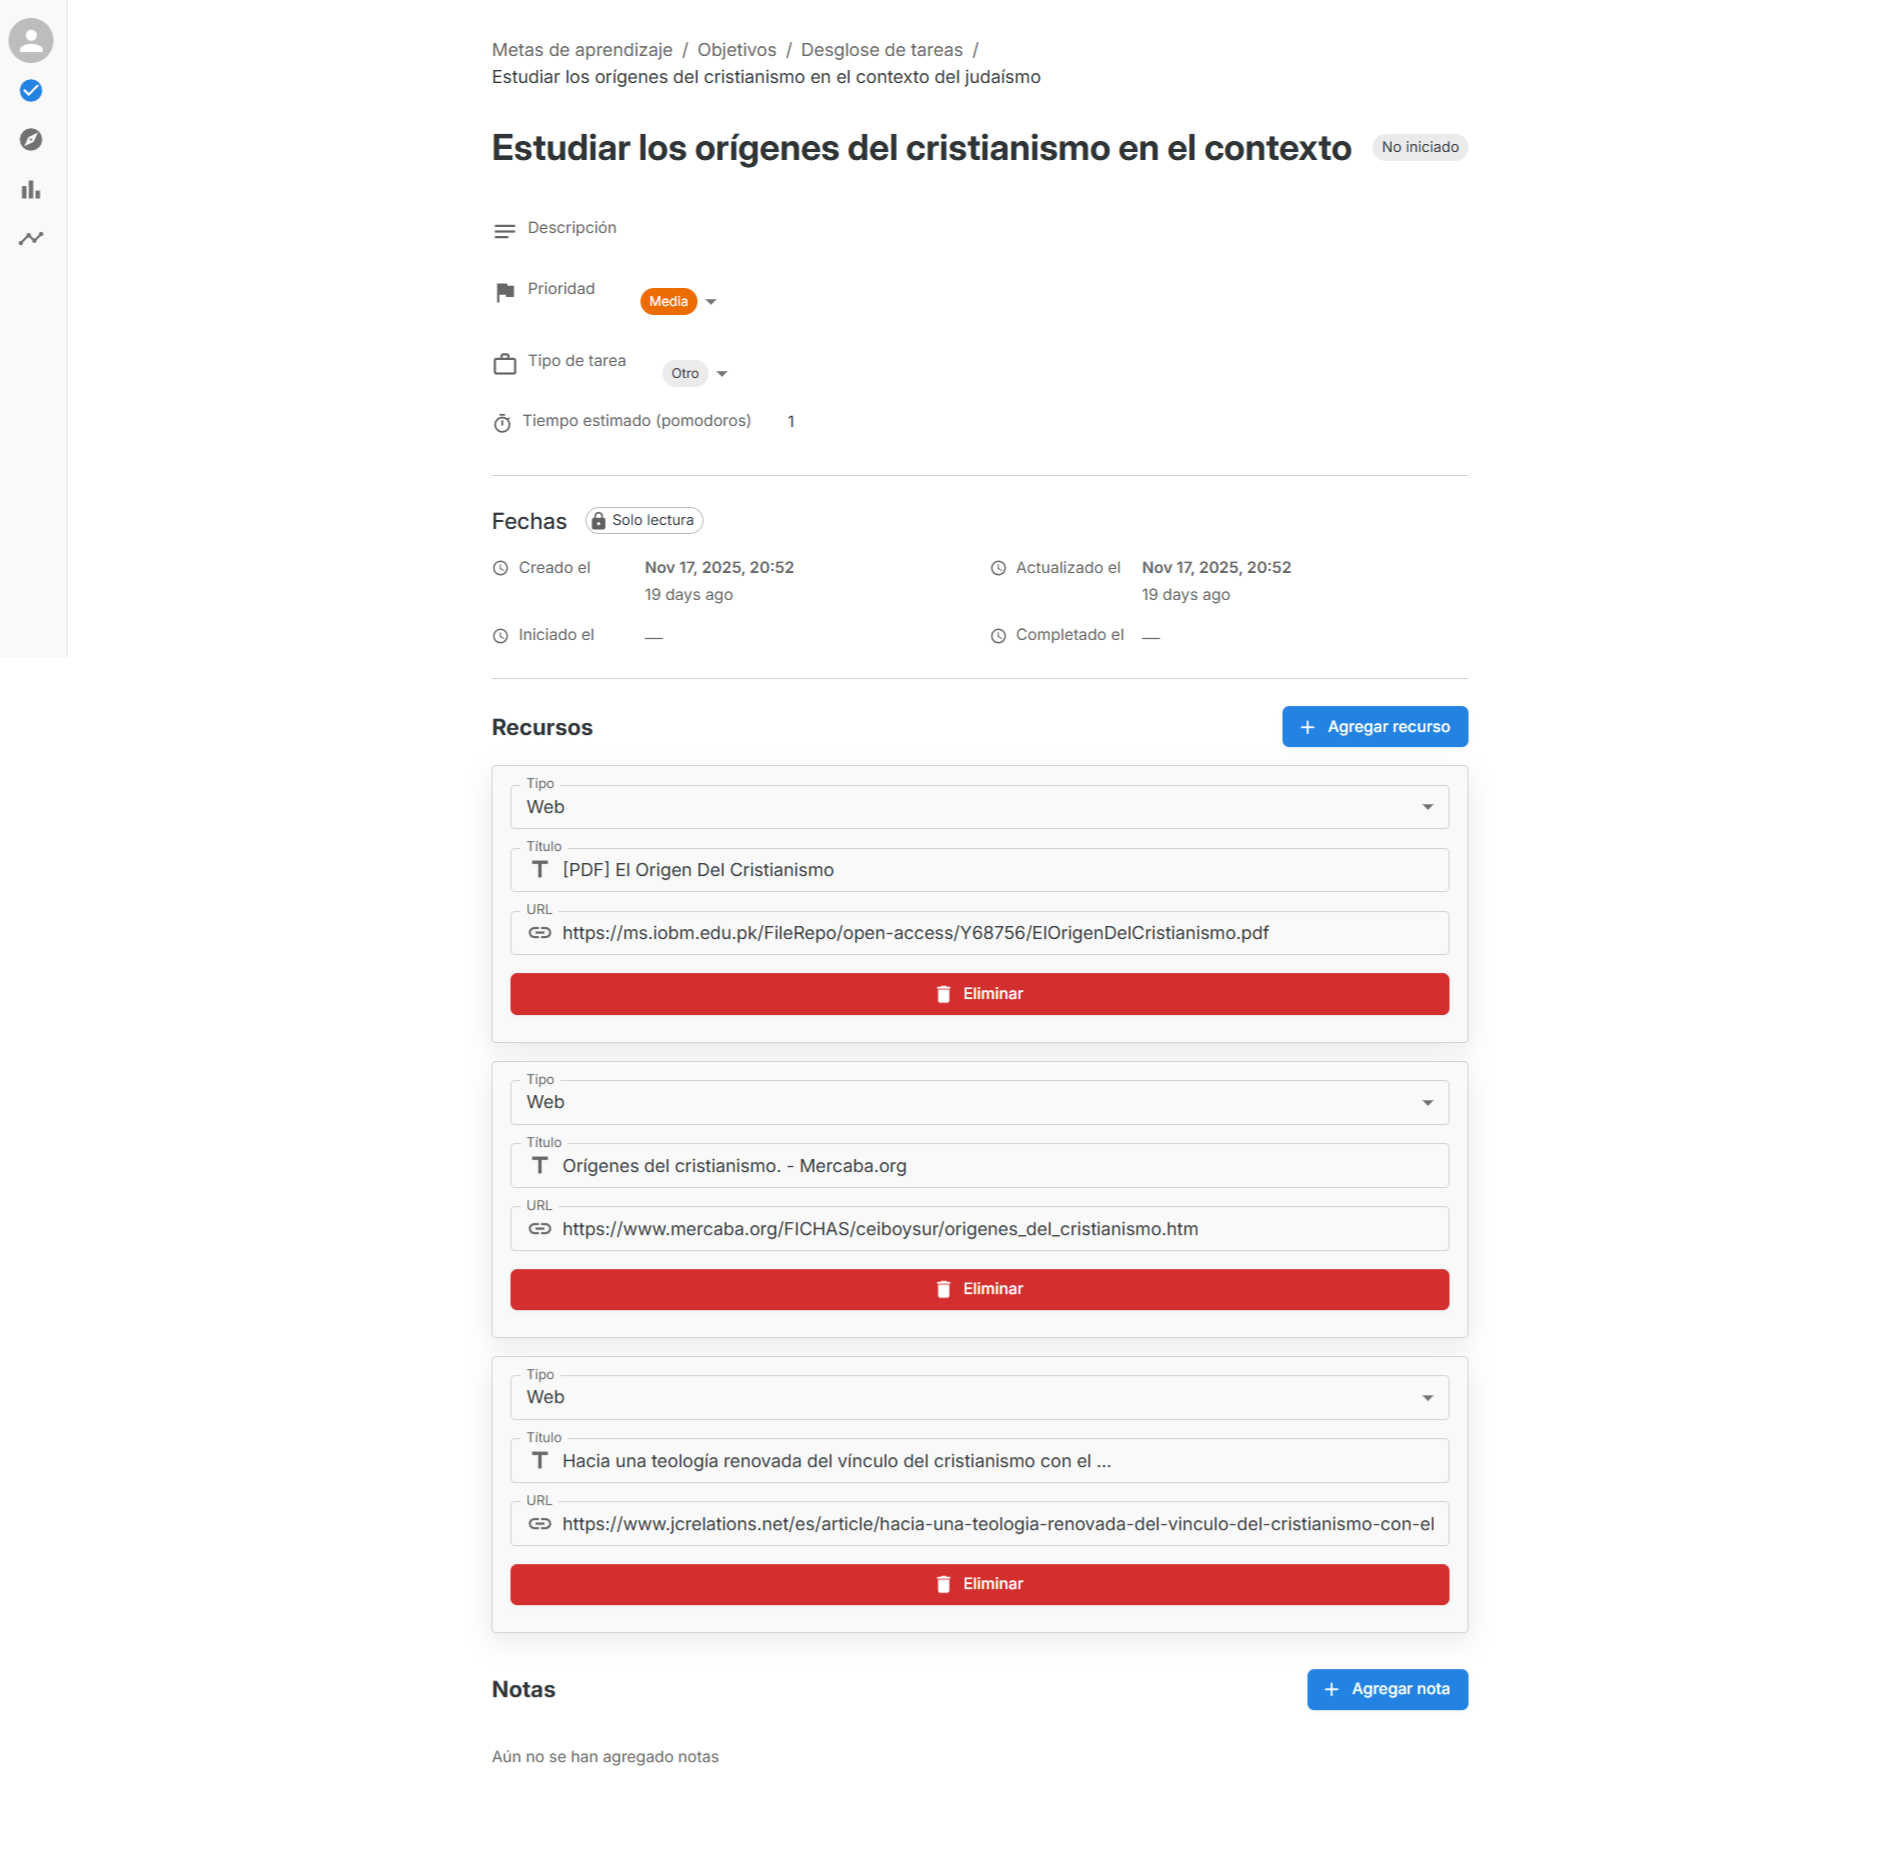
\includegraphics[width=0.95\textwidth]{Figuras/interfaces_AaA/plan_accionable_detalle_tarea.png}
\caption{Detalle de una tarea del plan accionable, incluyendo los recursos transferidos automáticamente desde el roadmap.}
\label{fig:accionable-detalle-tarea}
\end{figure}

\noindent\textit{Descripción.} Cuando una tarea en el roadmap incluye recursos (enlaces, documentos, videos, artículos), estos se trasladan automáticamente a la tarea equivalente del plan accionable. Esta transferencia garantiza consistencia entre la fase de planificación visual y la fase de ejecución del aprendizaje.

% -------------------------------------------------
% Exploración de planes de aprendizaje públicos
% -------------------------------------------------
\subsection*{Exploración de planes de aprendizaje públicos}

\begin{figure}[H]
\centering
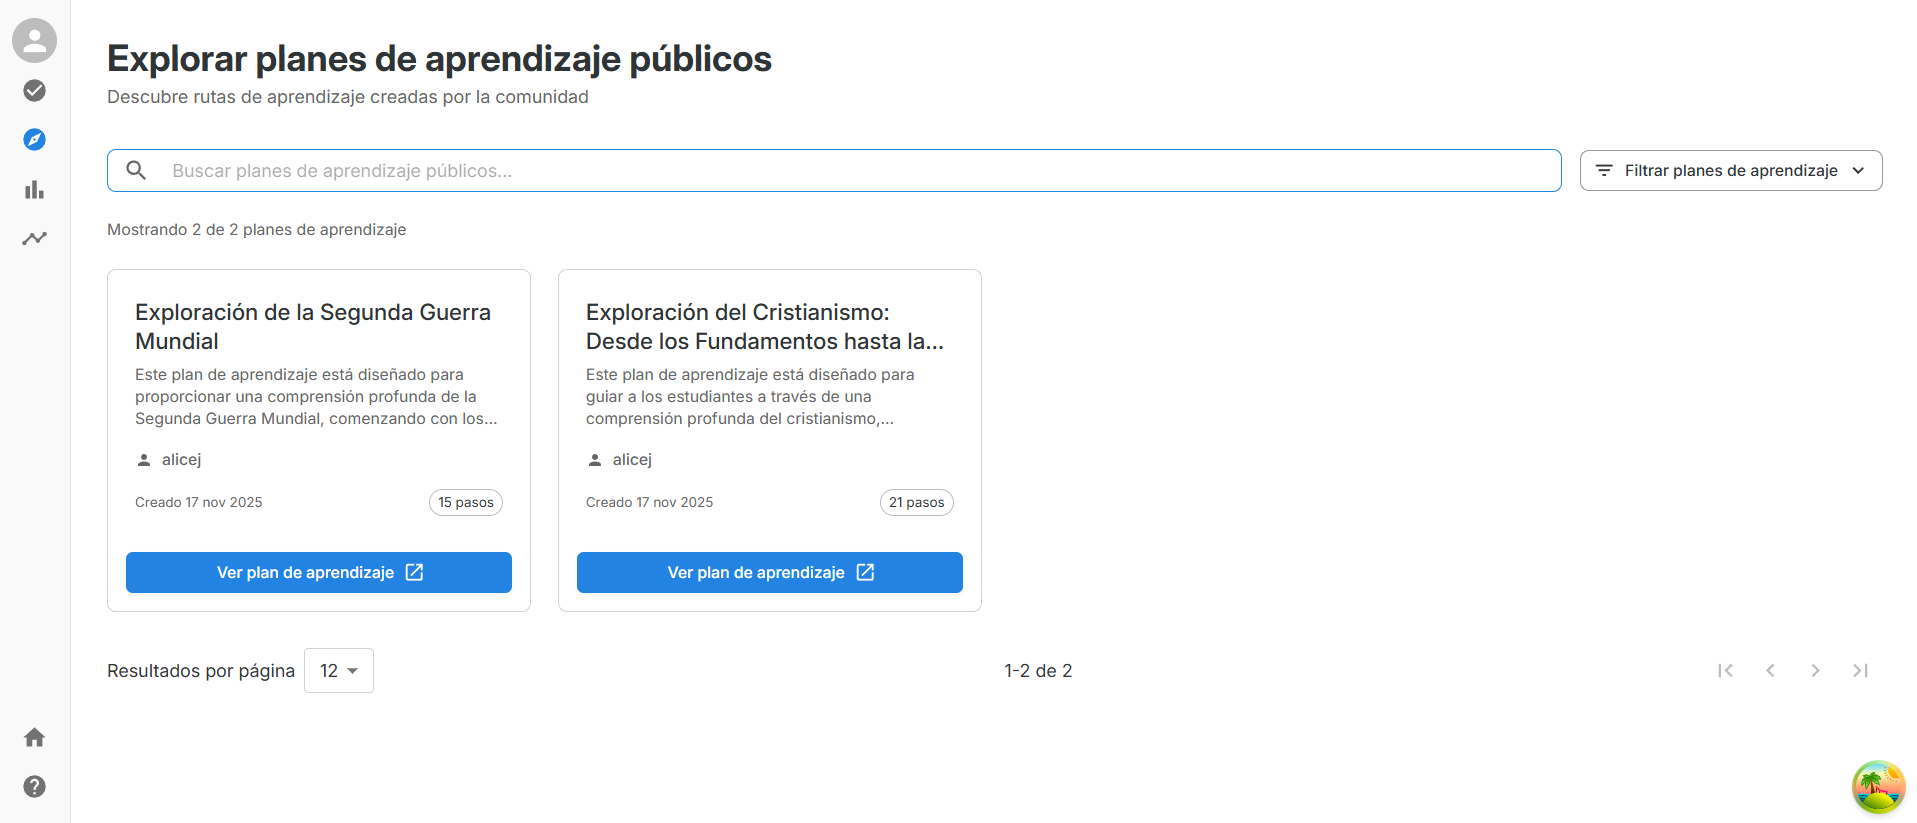
\includegraphics[width=0.95\textwidth]{Figuras/interfaces_AaA/exploracion_planes_publicos.png}
\caption{Listado de planes de aprendizaje públicos disponibles para exploración.}
\label{fig:exploracion-planes-publicos}
\end{figure}

\noindent\textit{Descripción.} La vista inicial muestra los planes públicos creados por la comunidad, junto con información relevante como título, autor, fecha de creación y número total de pasos del plan. Cada tarjeta permite acceder a la versión completa del plan para revisarlo antes de decidir su reutilización.

\begin{figure}[H]
\centering
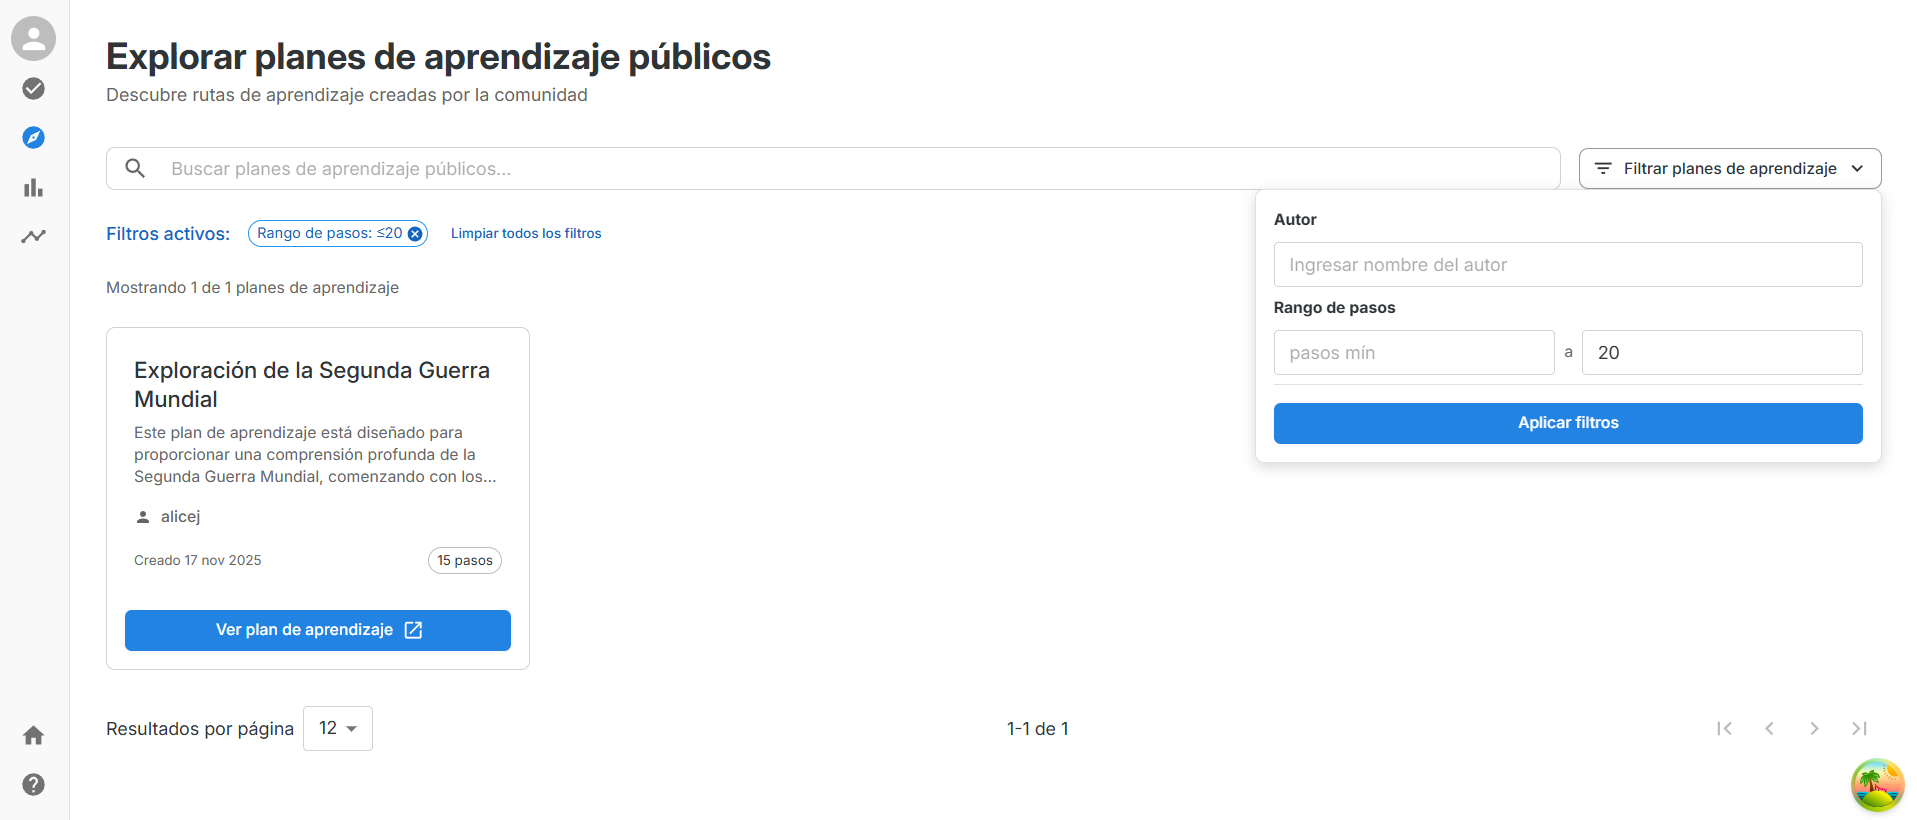
\includegraphics[width=0.95\textwidth]{Figuras/interfaces_AaA/exploracion_planes_publicos_filtros.png}
\caption{Aplicación de filtros por autor y rango de pasos en la exploración de planes públicos.}
\label{fig:exploracion-planes-publicos-filtros}
\end{figure}

\noindent\textit{Descripción.} El panel de filtrado permite acotar los resultados según criterios como el nombre del autor o el rango de pasos del plan. La interfaz actualiza la lista de resultados en función de los filtros aplicados, facilitando la búsqueda de modelos de referencia alineados con las necesidades del estudiante.

\subsection*{Copia y reutilización de planes públicos}

\begin{figure}[H]
\centering
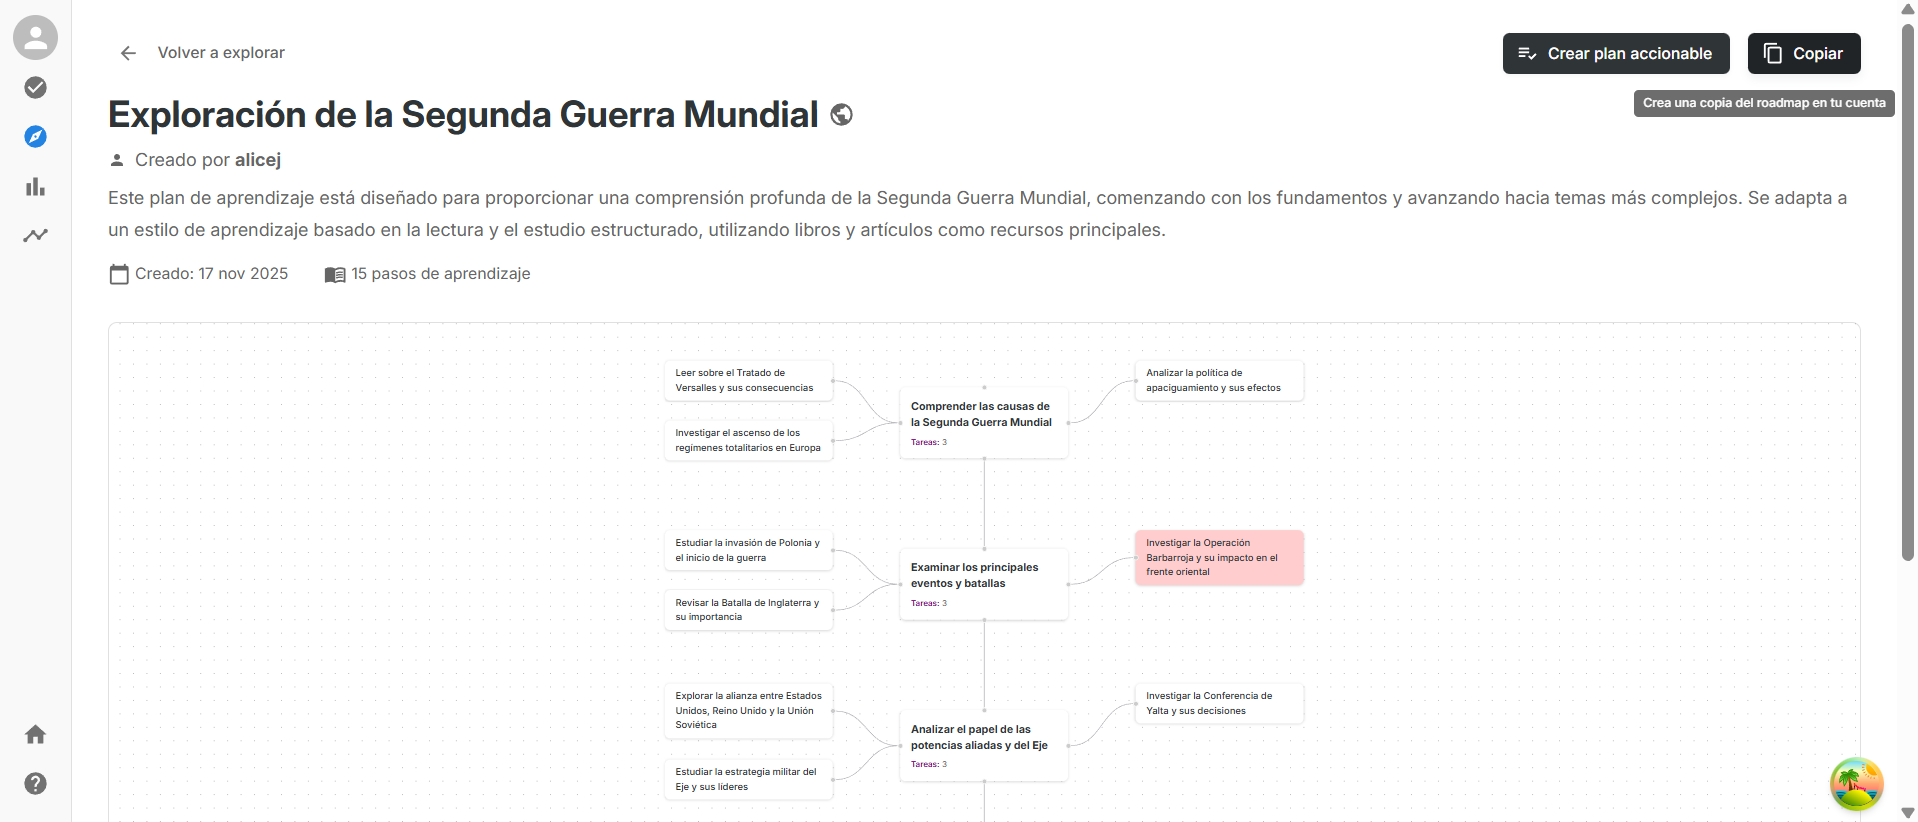
\includegraphics[width=0.95\textwidth]{Figuras/interfaces_AaA/copia_reutilizacion_planes_publicos.png}
\caption{Opción para copiar un plan de aprendizaje público hacia la cuenta del estudiante.}
\label{fig:copiar-plan-publico}
\end{figure}

\noindent\textit{Descripción.} El sistema permite que el estudiante tome cualquier plan de aprendizaje público y lo copie a su cuenta para reutilizarlo o adaptarlo a sus propias metas. Esta acción crea automáticamente una nueva versión del plan con \textbf{visibilidad privada}, asegurando que solo el estudiante pueda editarla o reorganizarla según sus necesidades.
\\
\\

\begin{figure}[H]
\centering
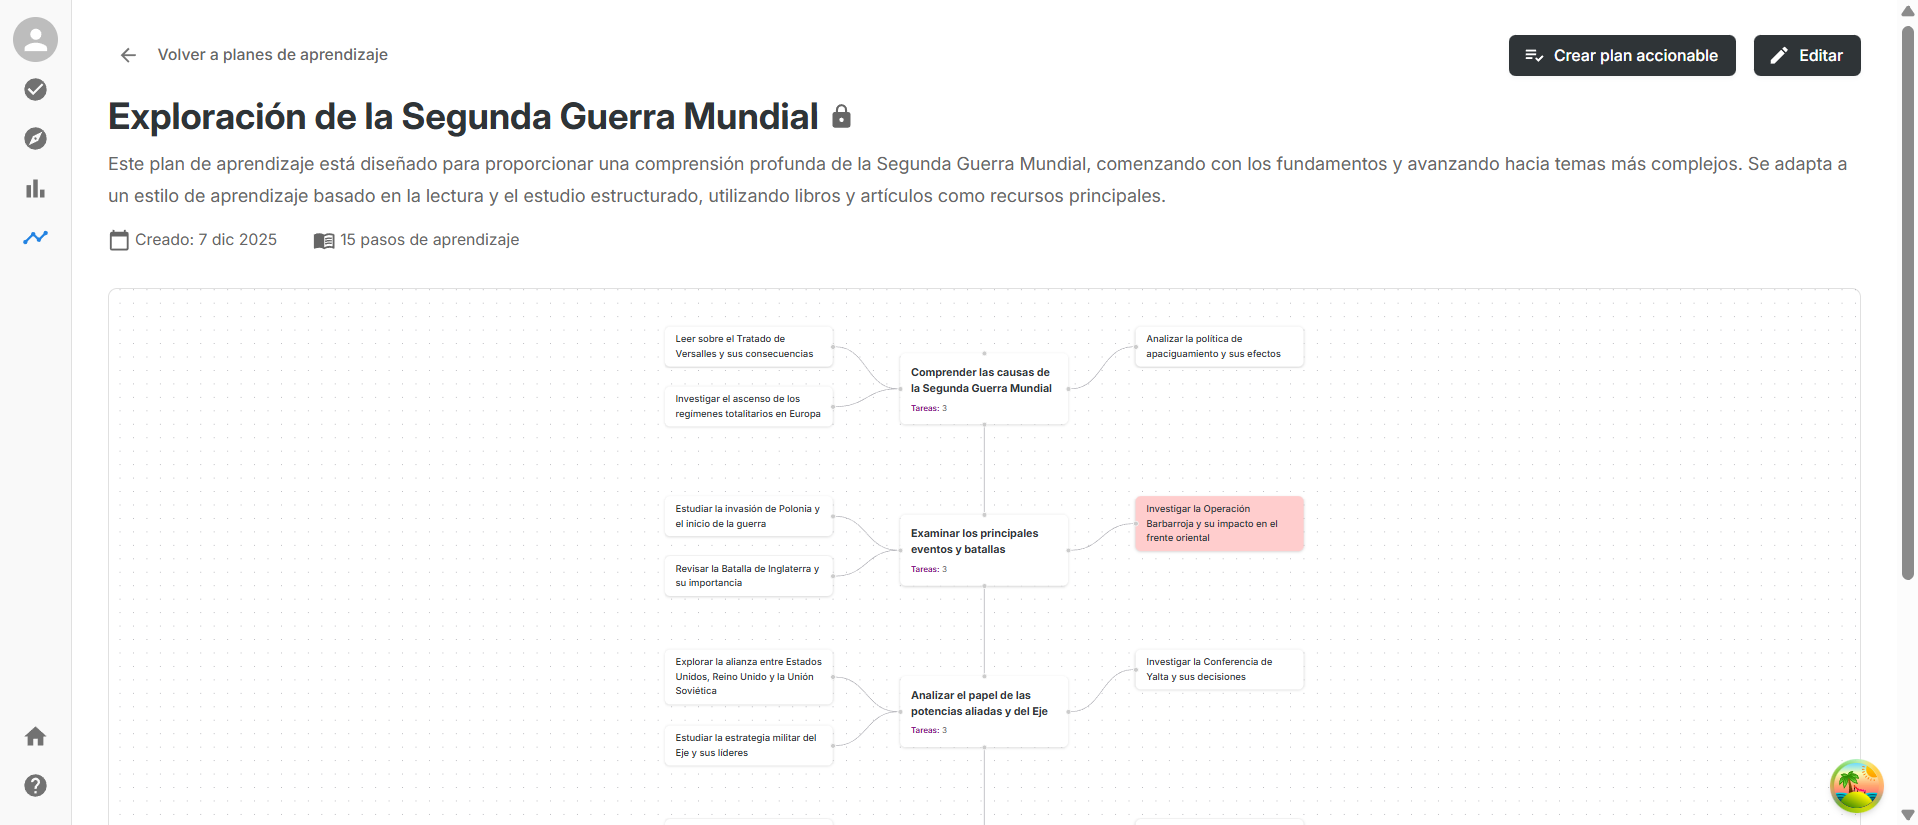
\includegraphics[width=0.95\textwidth]{Figuras/interfaces_AaA/plan_publico_copiado_en_cuenta.png}
\caption{Plan público copiado, ahora disponible como plan privado en la cuenta del estudiante.}
\label{fig:plan-publico-copiado}
\end{figure}

\noindent\textit{Descripción.} Una vez copiado, el plan aparece dentro del listado personal de metas de aprendizaje del estudiante, donde puede modificar objetivos, reorganizar tareas o transformar el plan en un roadmap visual si así lo requiere.

% -------------------------------------------------
\subsection*{Gestión de objetivos y tareas}
% -------------------------------------------------

\noindent Esta actividad se apoya en las mismas interfaces del editor visual y del plan accionable ya presentadas en las secciones anteriores, por lo que no se incluyen figuras adicionales.

% -------------------------------------------------
\subsection*{Seguimiento del progreso mediante Kanban}
% -------------------------------------------------
\noindent\textit{Descripción.} El tablero Kanban forma parte de la interfaz de detalle del objetivo dentro del plan accionable. En la Figura~\ref{fig:accionable-detalle-objetivo} se muestra cómo las tareas derivadas del roadmap se distribuyen automáticamente en columnas que reflejan su estado actual, facilitando el seguimiento del proceso de estudio.

% -------------------------------------------------
\subsection*{Desarrollo de tareas de aprendizaje}
% -------------------------------------------------
\noindent\textit{Descripción.} La Figura~\ref{fig:accionable-detalle-tarea} muestra la interfaz de detalle de una tarea dentro del plan accionable. Desde esta vista, el estudiante puede consultar los recursos transferidos automáticamente desde el roadmap, mientras que el cambio de estado de la tarea (iniciada, en pausa o completada) se realiza moviendo la tarjeta dentro del tablero Kanban.

% -------------------------------------------------
\subsection*{Agregación de recursos a las tareas}
% -------------------------------------------------

% (1) Formulario para agregar un recurso
\begin{figure}[H]
\centering
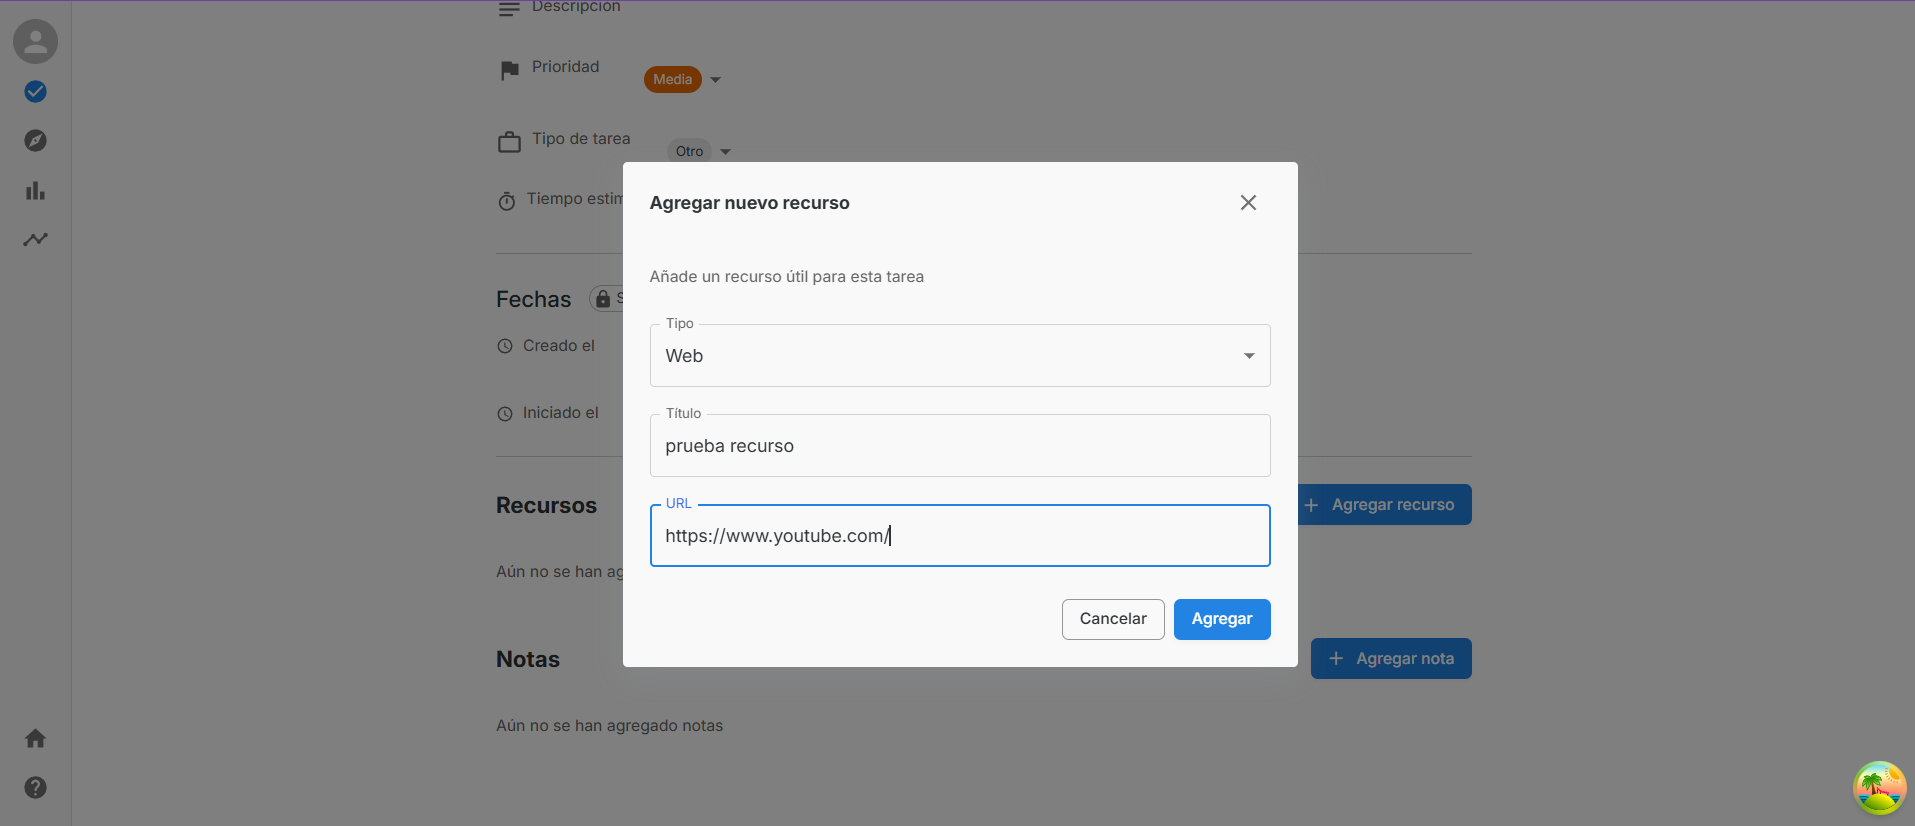
\includegraphics[width=0.95\textwidth]{Figuras/interfaces_AaA/agregar_recurso_tarea.png}
\caption{Formulario para agregar un nuevo recurso a una tarea dentro del plan accionable.}
\label{fig:agregar-recurso-tarea}
\end{figure}

\noindent\textit{Descripción.} Al seleccionar la opción \textit{Agregar recurso}, se despliega un formulario que permite especificar el tipo de recurso, su título y su URL. Al confirmar, el recurso queda asociado a la tarea.

% (2) Listado de recursos agregados
\begin{figure}[H]
\centering
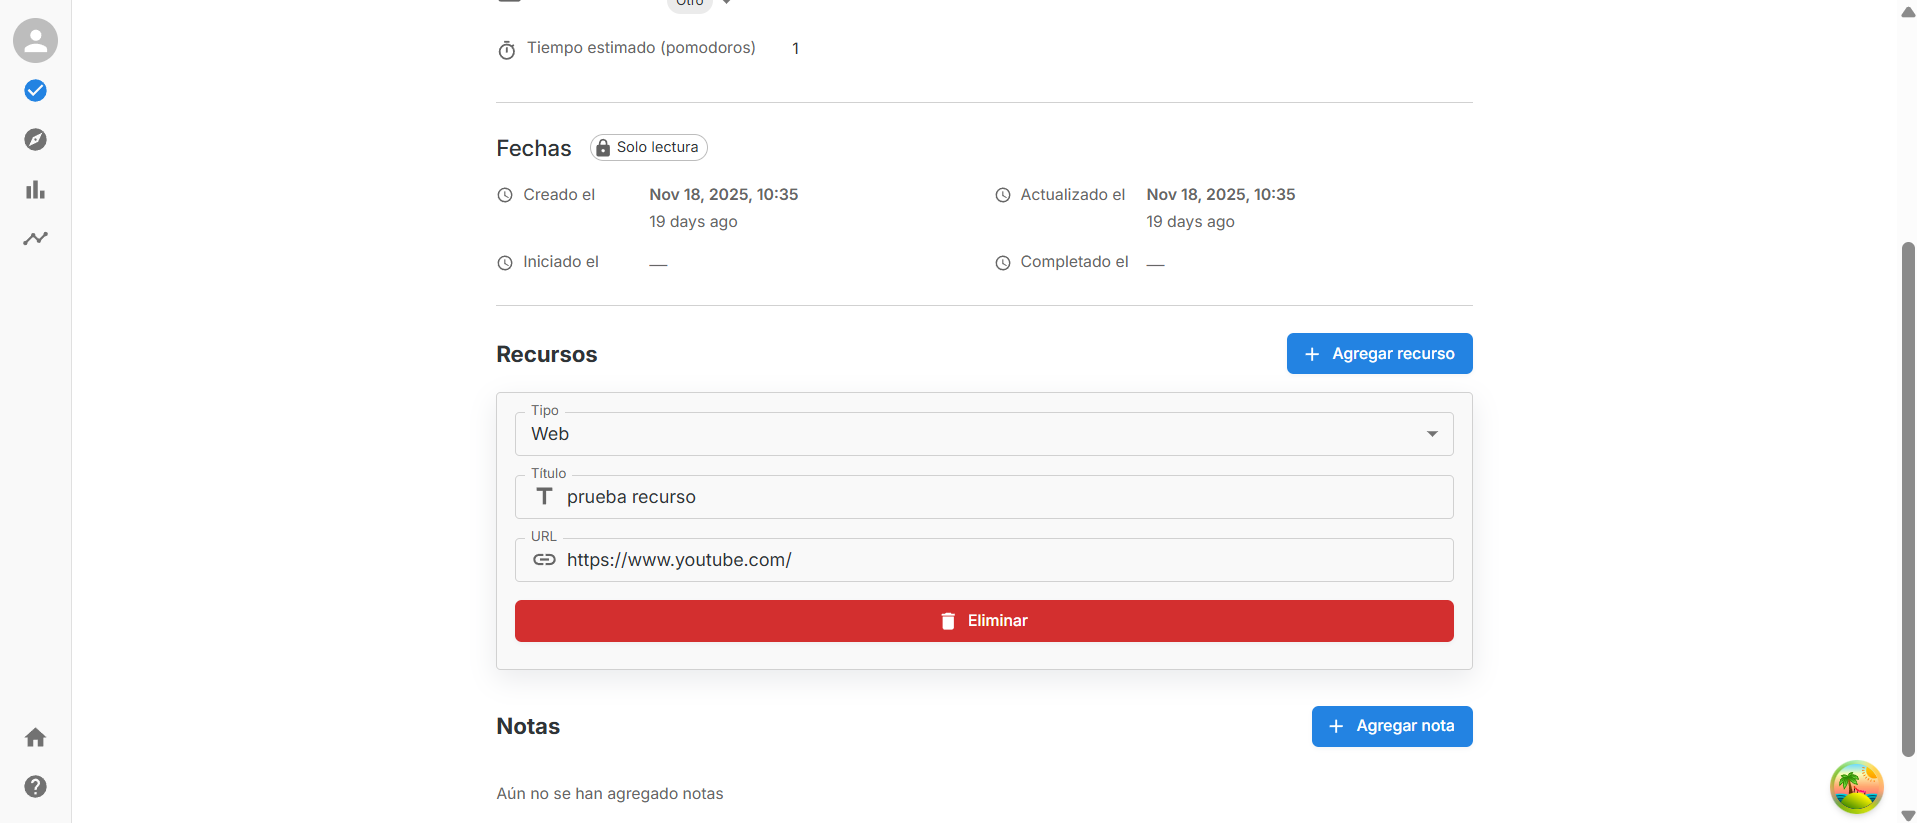
\includegraphics[width=0.95\textwidth]{Figuras/interfaces_AaA/tarea_recurso_listado.png}
\caption{Listado de recursos asociados a una tarea, con opciones para editarlos o eliminarlos.}
\label{fig:listado-recursos-tarea}
\end{figure}

\noindent\textit{Descripción.} Una vez agregado, el recurso aparece en el listado de la tarea, donde puede ser consultado, modificado o eliminado. Esta vista permite al estudiante gestionar de manera flexible los materiales que apoyan su proceso de aprendizaje.

% -------------------------------------------------
\subsection*{Registro de notas personales por tarea}
% -------------------------------------------------

% (1) Agregar nueva nota
\begin{figure}[H]
\centering
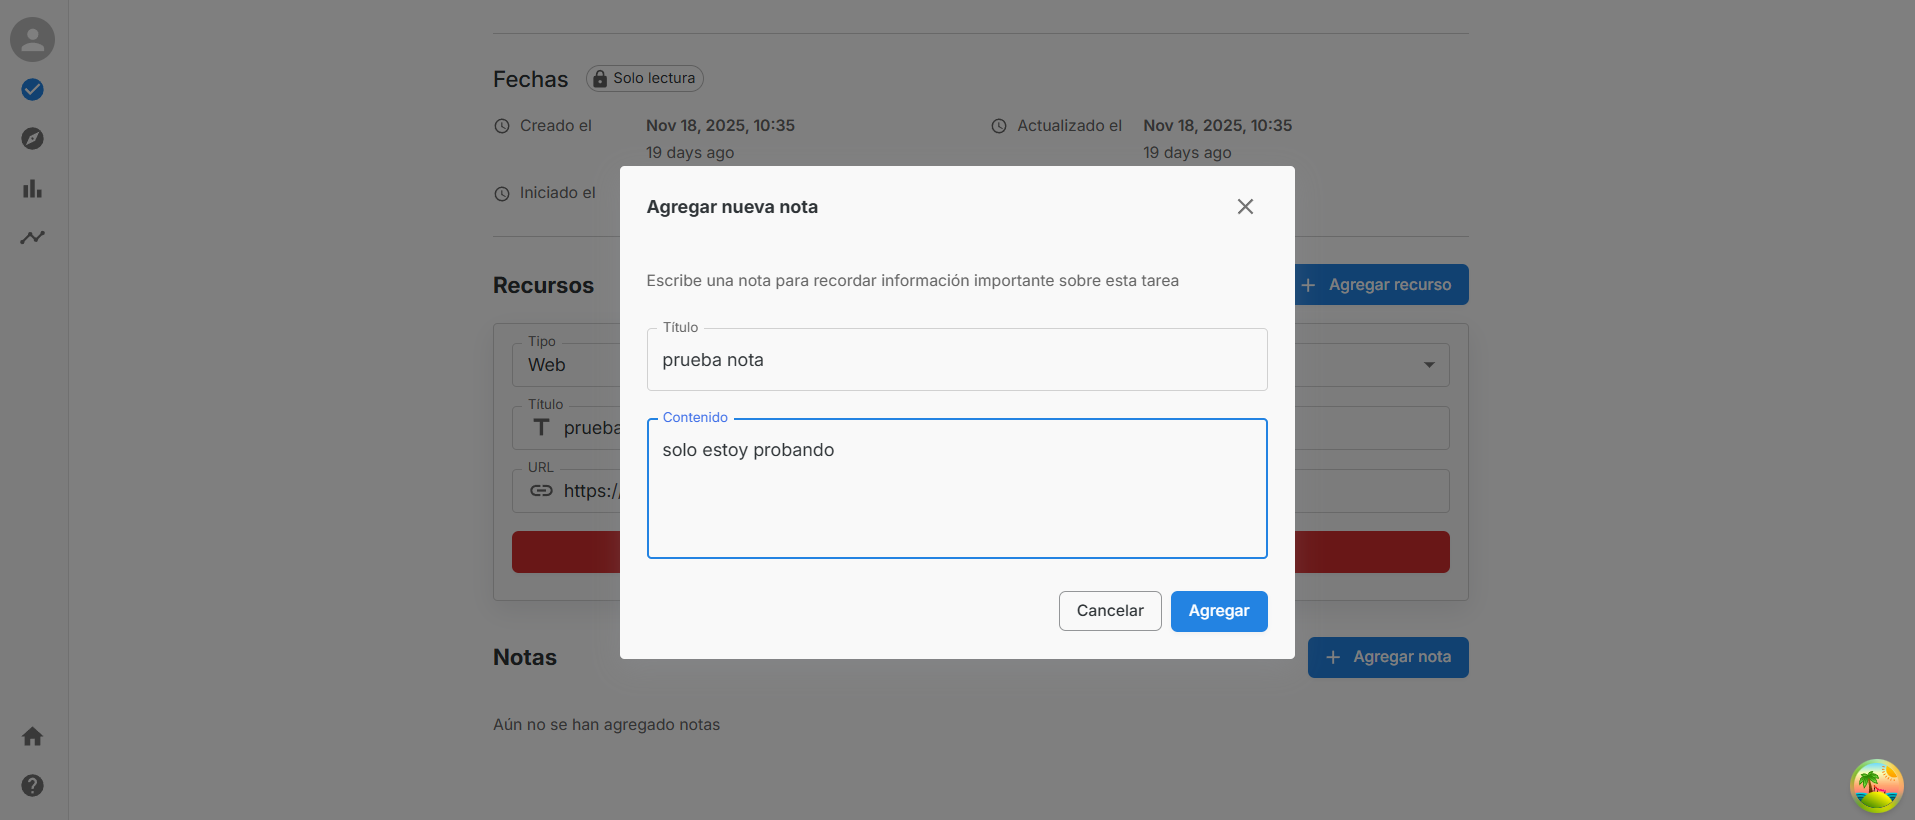
\includegraphics[width=0.95\textwidth]{Figuras/interfaces_AaA/tarea_agregar_nota.png}
\caption{Interfaz para agregar una nueva nota a una tarea.}
\label{fig:tarea-agregar-nota}
\end{figure}

\noindent\textit{Descripción.} La Figura~\ref{fig:tarea-agregar-nota} muestra el formulario utilizado para registrar una nota personal. El estudiante puede definir un título y un contenido, permitiendo documentar información útil para el avance de la tarea.

% (2) Listado y gestión de notas existentes
\begin{figure}[H]
\centering
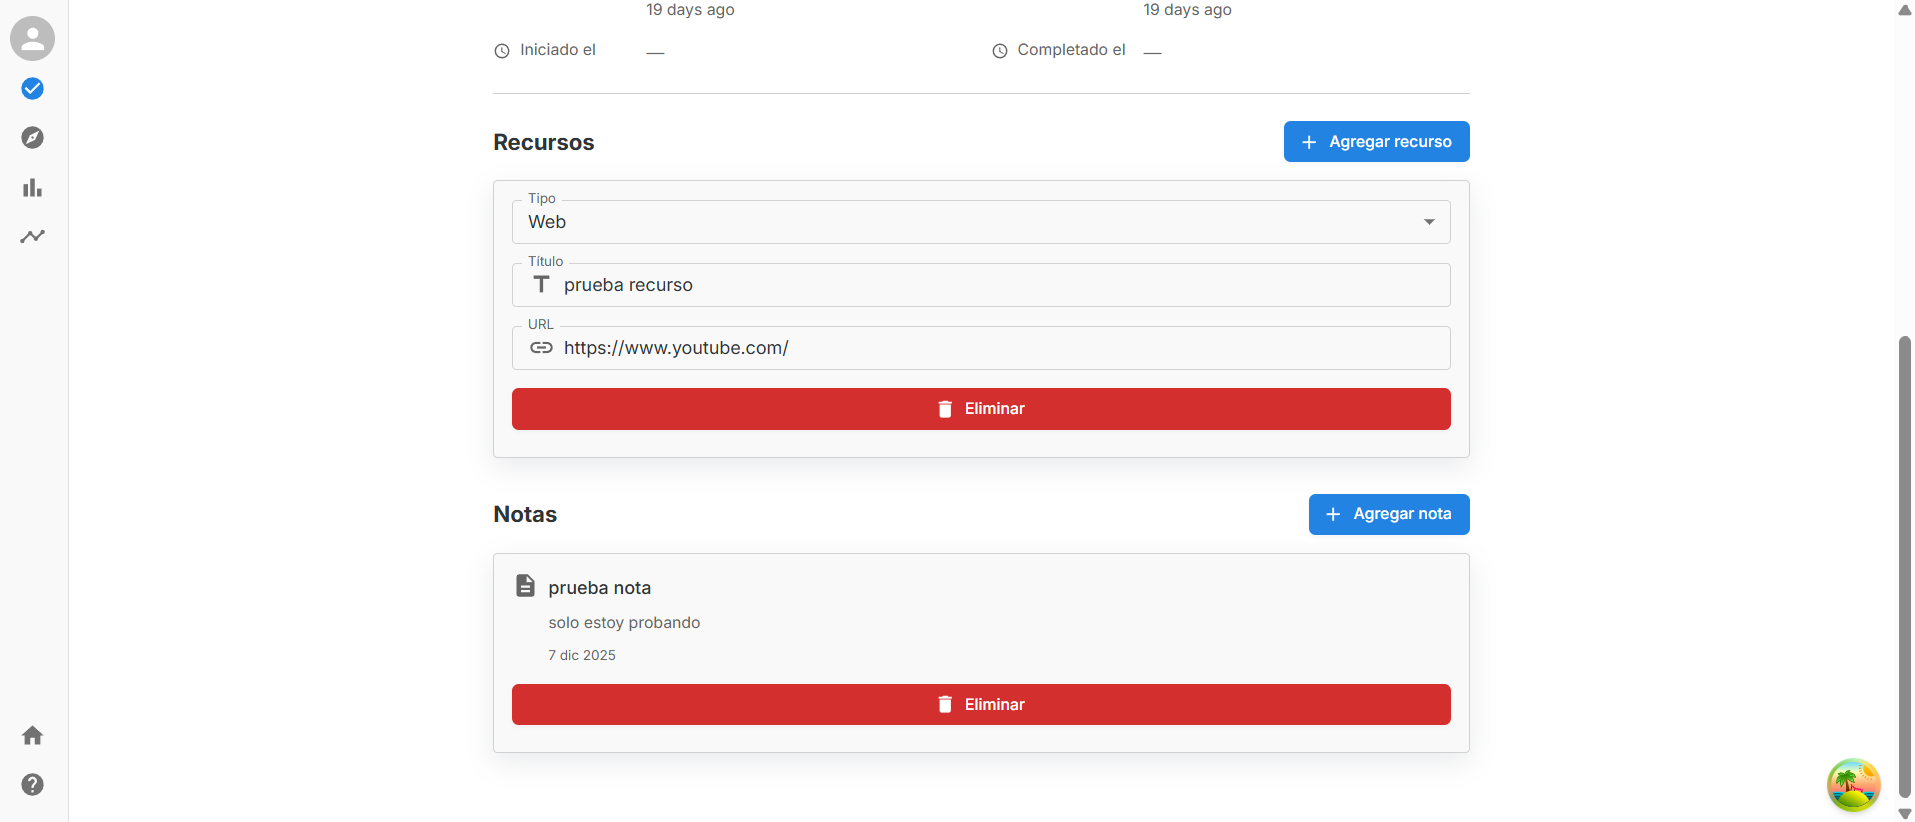
\includegraphics[width=0.95\textwidth]{Figuras/interfaces_AaA/tarea_listado_notas.png}
\caption{Listado de notas asociadas a una tarea, con opciones para su gestión.}
\label{fig:tarea-listado-notas}
\end{figure}

\noindent\textit{Descripción.} La Figura~\ref{fig:tarea-listado-notas} ilustra cómo las notas se presentan dentro del detalle de la tarea. Desde esta vista, el estudiante puede revisar o eliminar cada nota según requiera su proceso de estudio.

% -------------------------------------------------
\subsection*{Autoevaluación y reflexión guiada al finalizar una tarea}
% -------------------------------------------------

Al mover una tarea a la columna \textit{Hecho} dentro del tablero Kanban, el sistema presenta un formulario de reflexión orientado a promover la autorregulación del aprendizaje. Este formulario debe completarse para confirmar la finalización de la tarea; en caso de cancelarse, la tarea regresa automáticamente al estado previo, garantizando que toda actividad marcada como completada cuente con una reflexión asociada.

% (1) Reflexión: entorno e intención de aprendizaje
\begin{figure}[H]
\centering
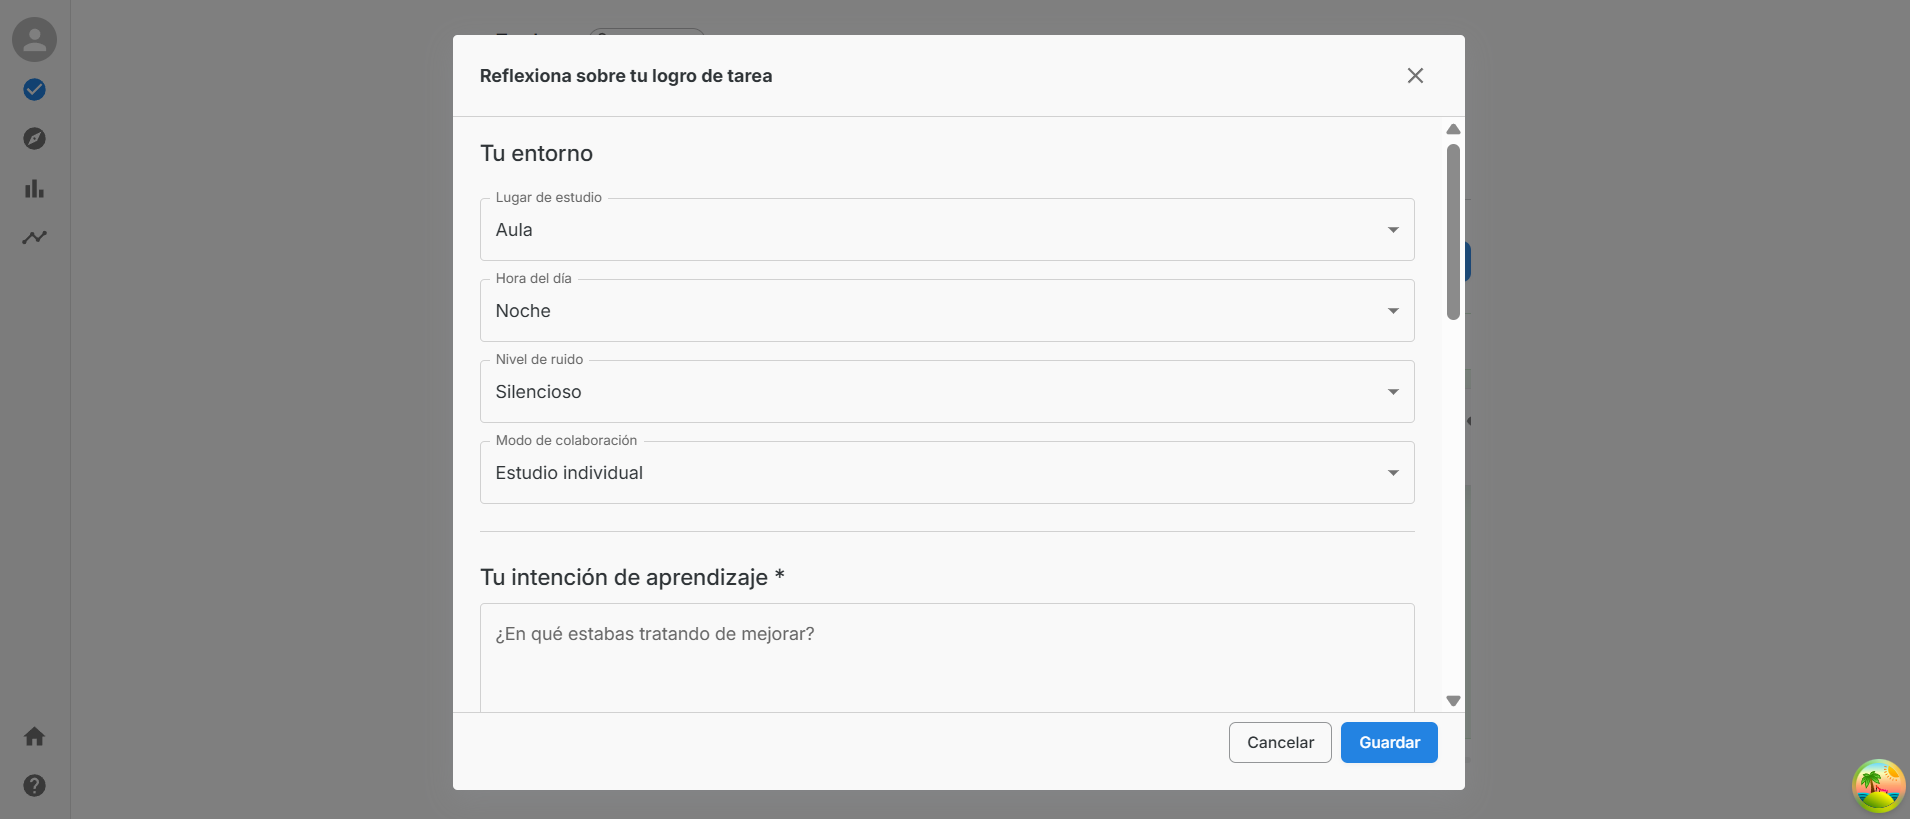
\includegraphics[width=0.95\textwidth]{Figuras/interfaces_AaA/reflexion_tarea_entorno.png}
\caption{Primera sección del formulario de reflexión: entorno y meta de aprendizaje.}
\label{fig:reflexion-tarea-entorno}
\end{figure}

\noindent\textit{Descripción.} La primera sección recopila información contextual sobre la sesión de estudio, incluyendo el lugar, la hora del día, el nivel de ruido y el modo de colaboración. También solicita la intención de aprendizaje asociada a la tarea, permitiendo al estudiante clarificar el propósito de su actividad.

% (2) Reflexión: experiencia durante la tarea
\begin{figure}[H]
\centering
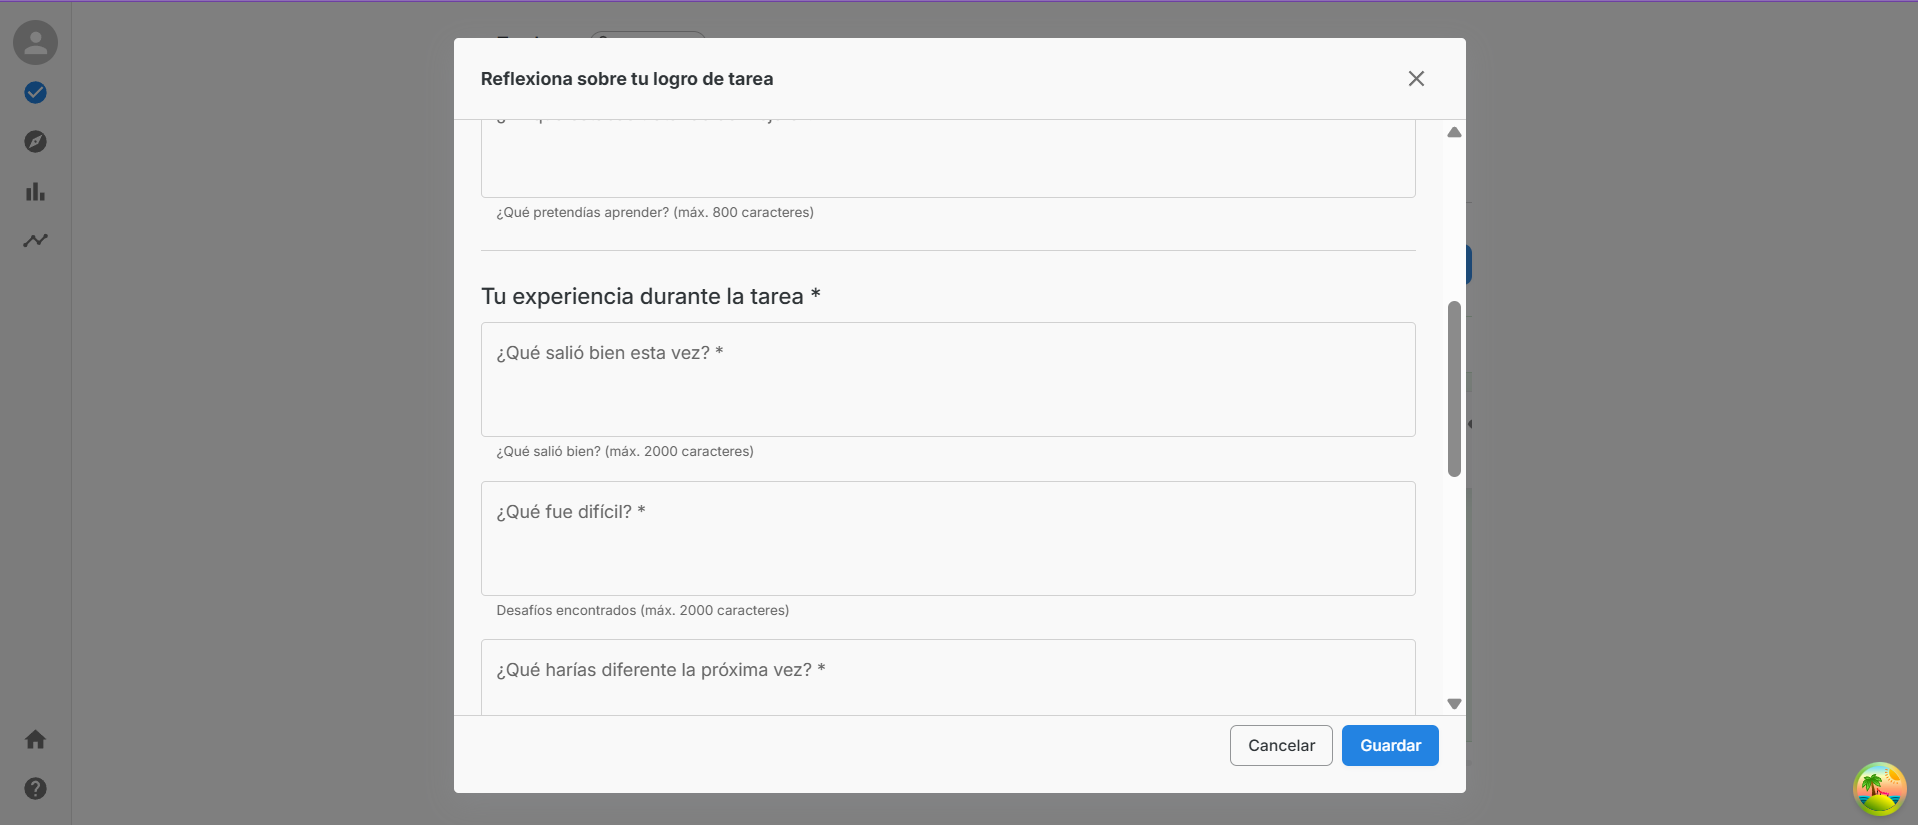
\includegraphics[width=0.95\textwidth]{Figuras/interfaces_AaA/reflexion_tarea_experiencia.png}
\caption{Segunda sección del formulario de reflexión: experiencia durante la tarea.}
\label{fig:reflexion-tarea-experiencia}
\end{figure}

\noindent\textit{Descripción.} En esta sección, el estudiante describe su experiencia al realizar la tarea, destacando qué salió bien, qué resultó difícil y qué acciones podría mejorar en futuras actividades. Este análisis favorece la toma de conciencia sobre el propio proceso de aprendizaje.

% (3) Reflexión: nivel de esfuerzo, concentración y estrategias
\begin{figure}[H]
\centering
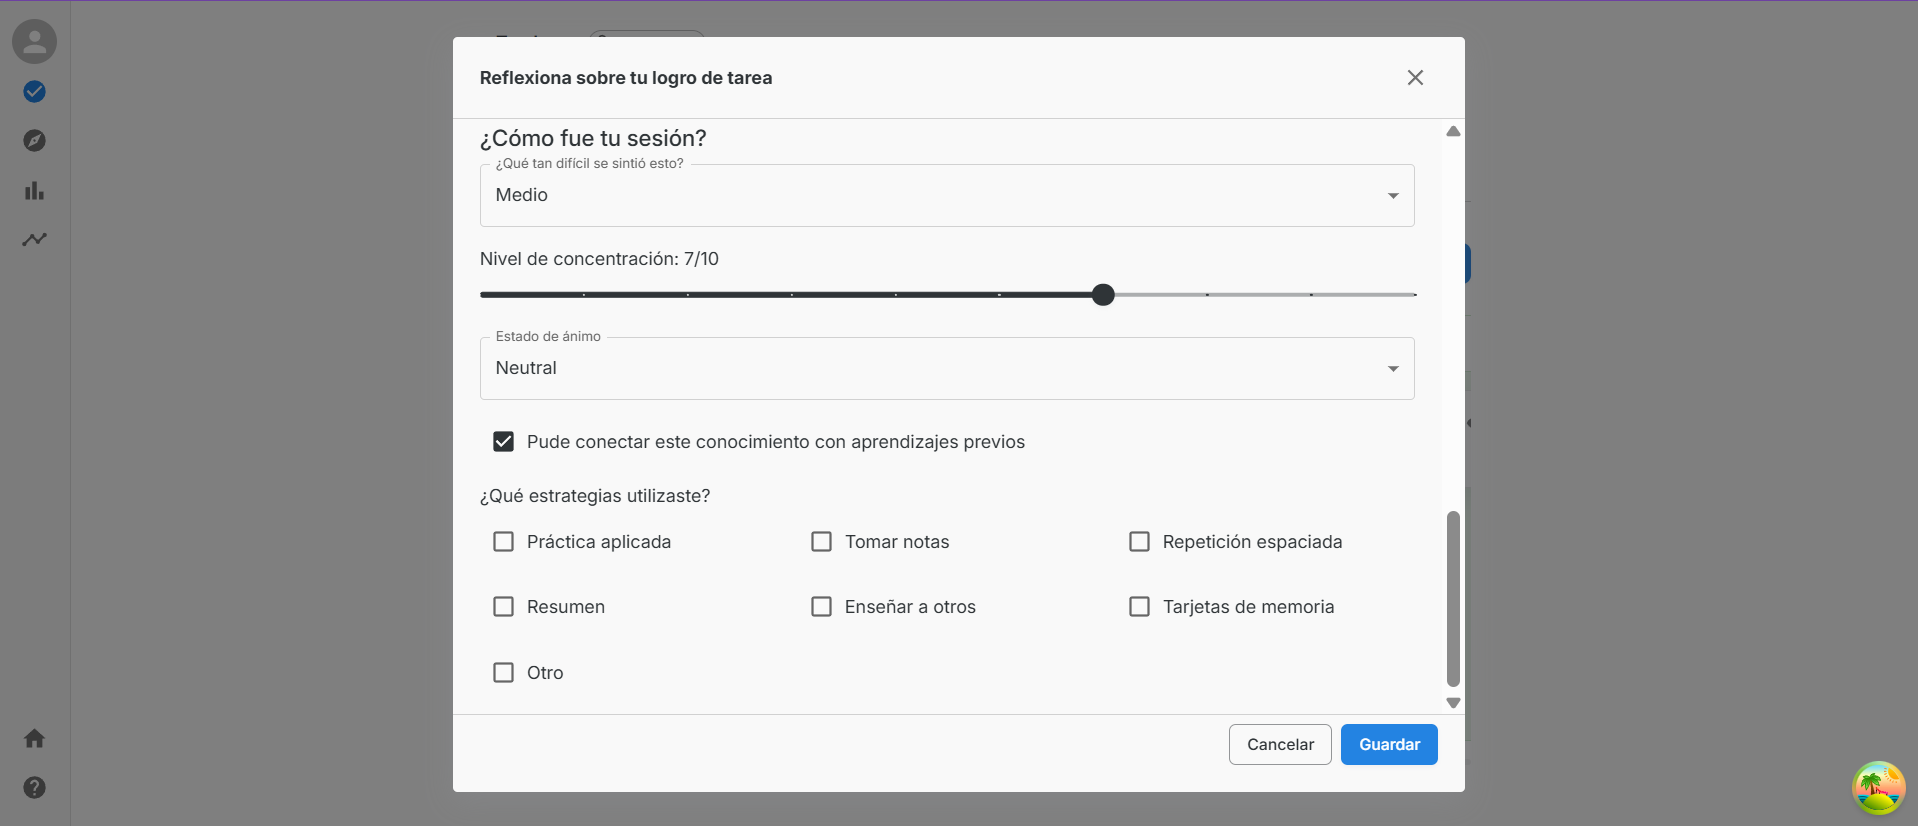
\includegraphics[width=0.95\textwidth]{Figuras/interfaces_AaA/reflexion_tarea_sesion.png}
\caption{Tercera sección del formulario de reflexión: nivel de esfuerzo, concentración, estado de ánimo y estrategias utilizadas.}
\label{fig:reflexion-tarea-sesion}
\end{figure}

\noindent\textit{Descripción.} La sección final incluye una valoración subjetiva sobre el nivel de dificultad, la concentración y el estado de ánimo del estudiante. Además, permite registrar las estrategias de aprendizaje utilizadas y si el nuevo conocimiento pudo conectarse con experiencias previas, reforzando así habilidades metacognitivas esenciales.

% -------------------------------------------------
\subsection*{Acceso a reportes de aprendizaje}
% -------------------------------------------------
% (1) Lista general de informes de aprendizaje
\begin{figure}[H]
\centering
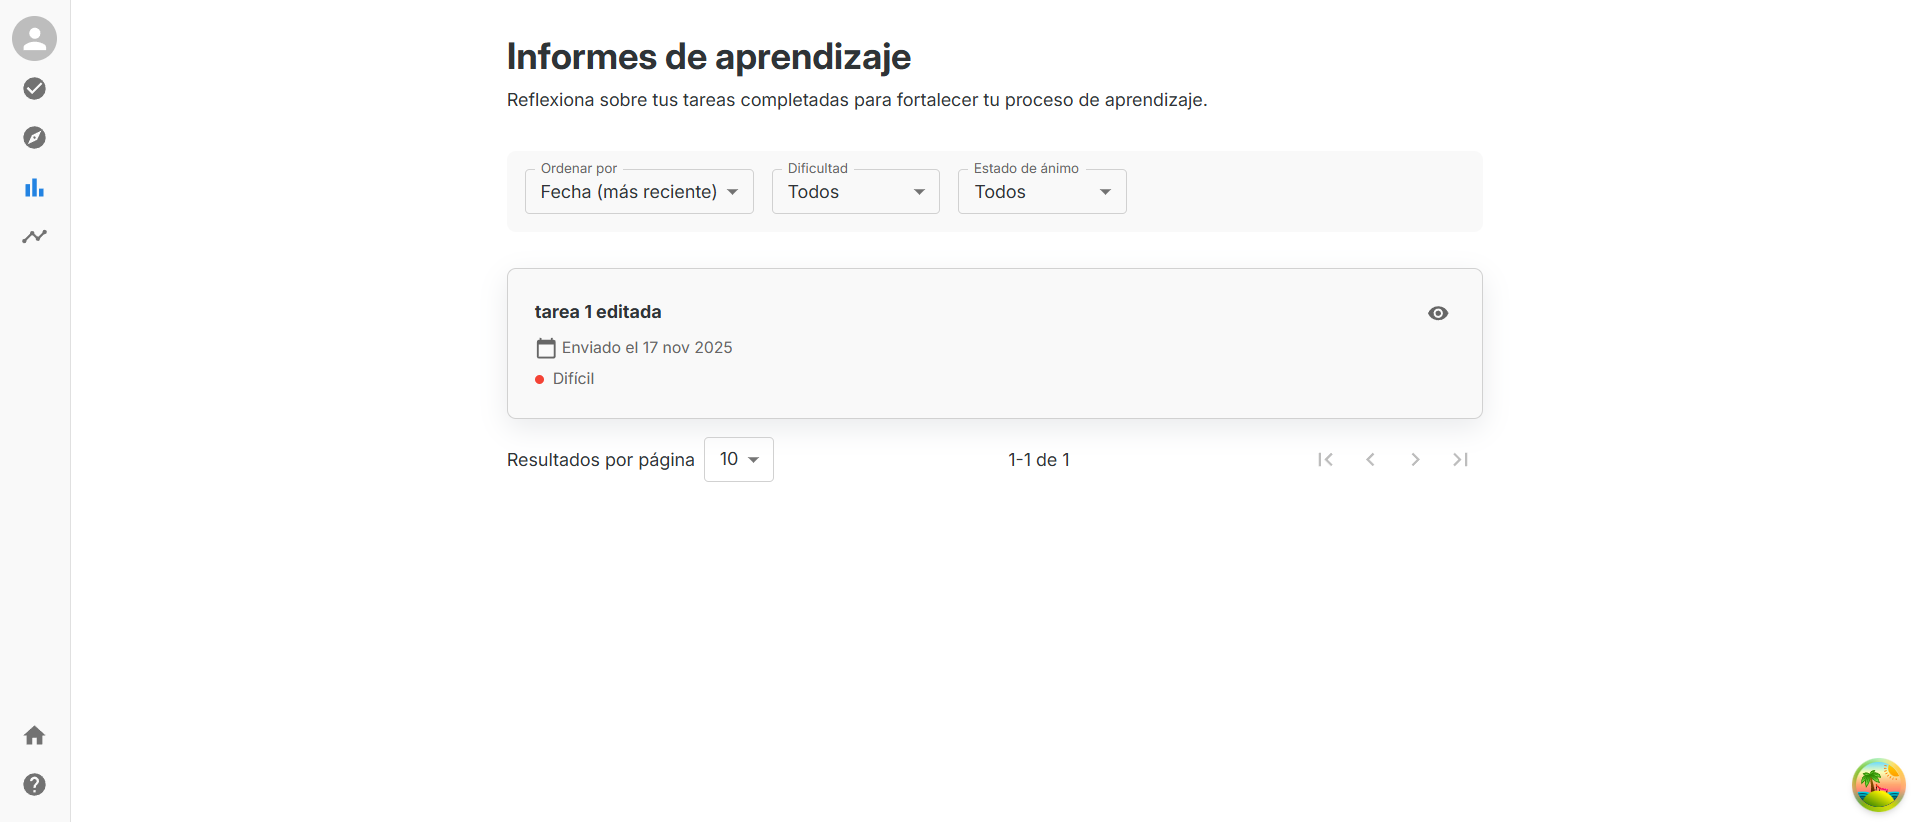
\includegraphics[width=0.95\textwidth]{Figuras/interfaces_AaA/reportes_lista_general.png}
\caption{Listado general de informes de aprendizaje, con opciones de ordenamiento y filtrado.}
\label{fig:reportes-lista-general}
\end{figure}

\noindent\textit{Descripción.} 
La vista inicial presenta todas las autoevaluaciones enviadas, permitiendo ordenar los reportes por fecha y aplicar filtros adicionales que facilitan la exploración del historial de aprendizaje.

% (2) Lista filtrada sin resultados
\begin{figure}[H]
\centering
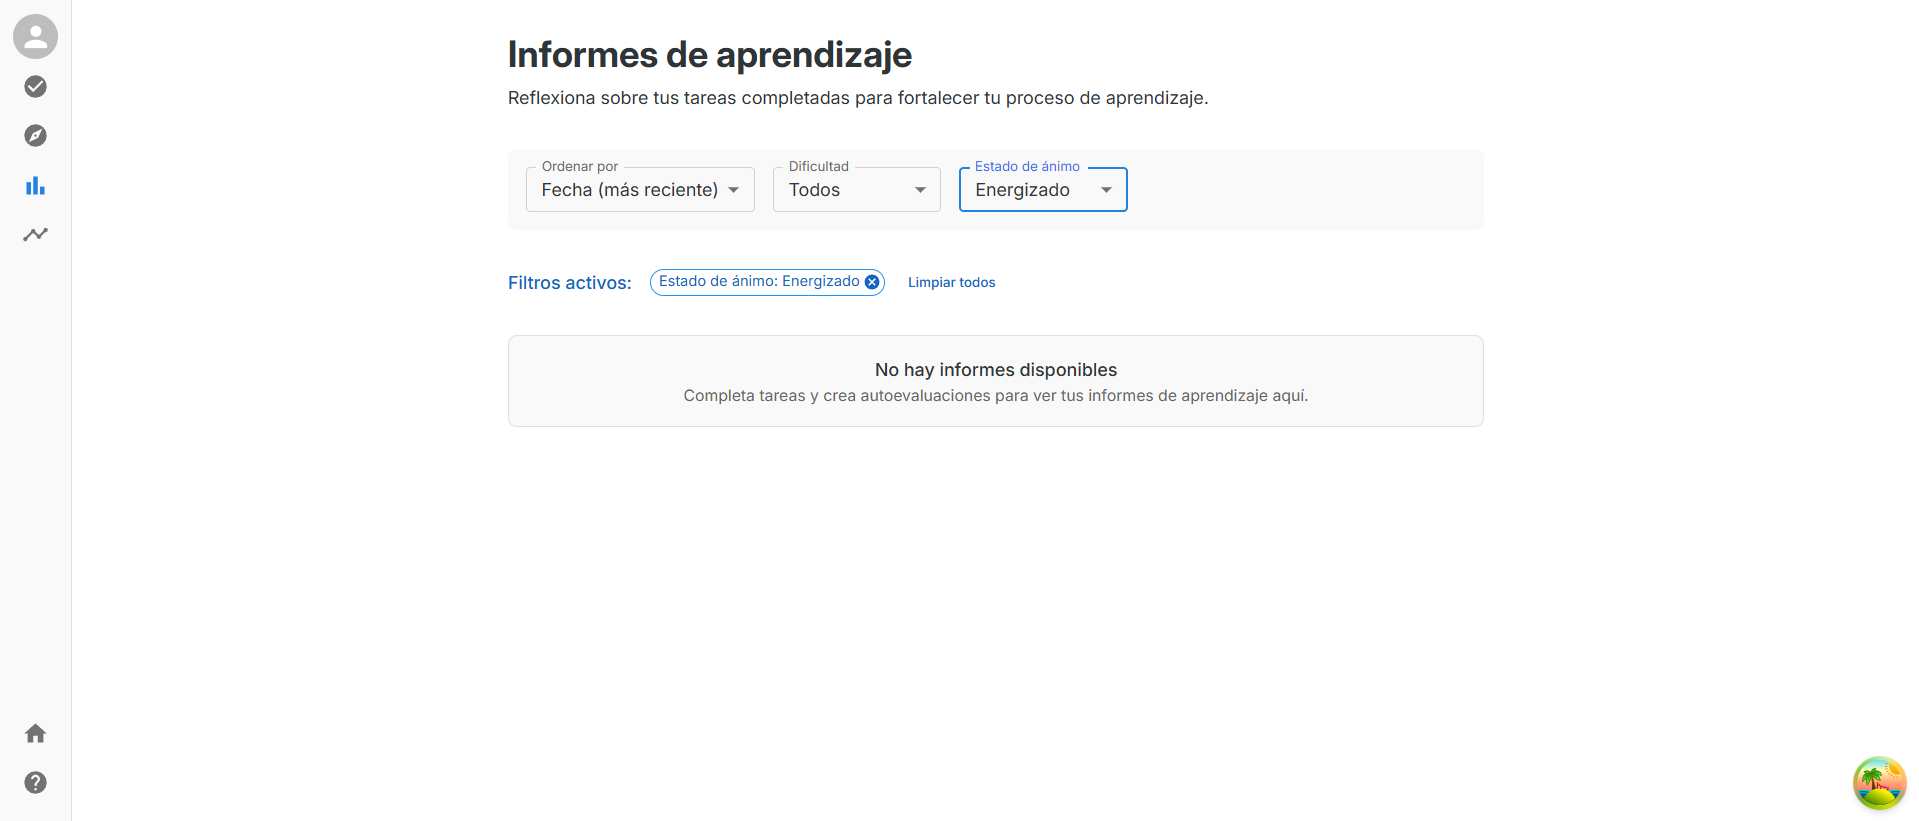
\includegraphics[width=0.95\textwidth]{Figuras/interfaces_AaA/reportes_sin_resultados.png}
\caption{Vista del módulo de reportes cuando los filtros aplicados no arrojan resultados.}
\label{fig:reportes-sin-resultados}
\end{figure}

\noindent\textit{Descripción.} 
Cuando ningún reporte coincide con los filtros seleccionados, el sistema informa al estudiante y lo invita a completar nuevas tareas y reflexiones para generar contenido en esta sección.

% (3) Vista detallada de un informe de aprendizaje
\begin{figure}[H]
\centering
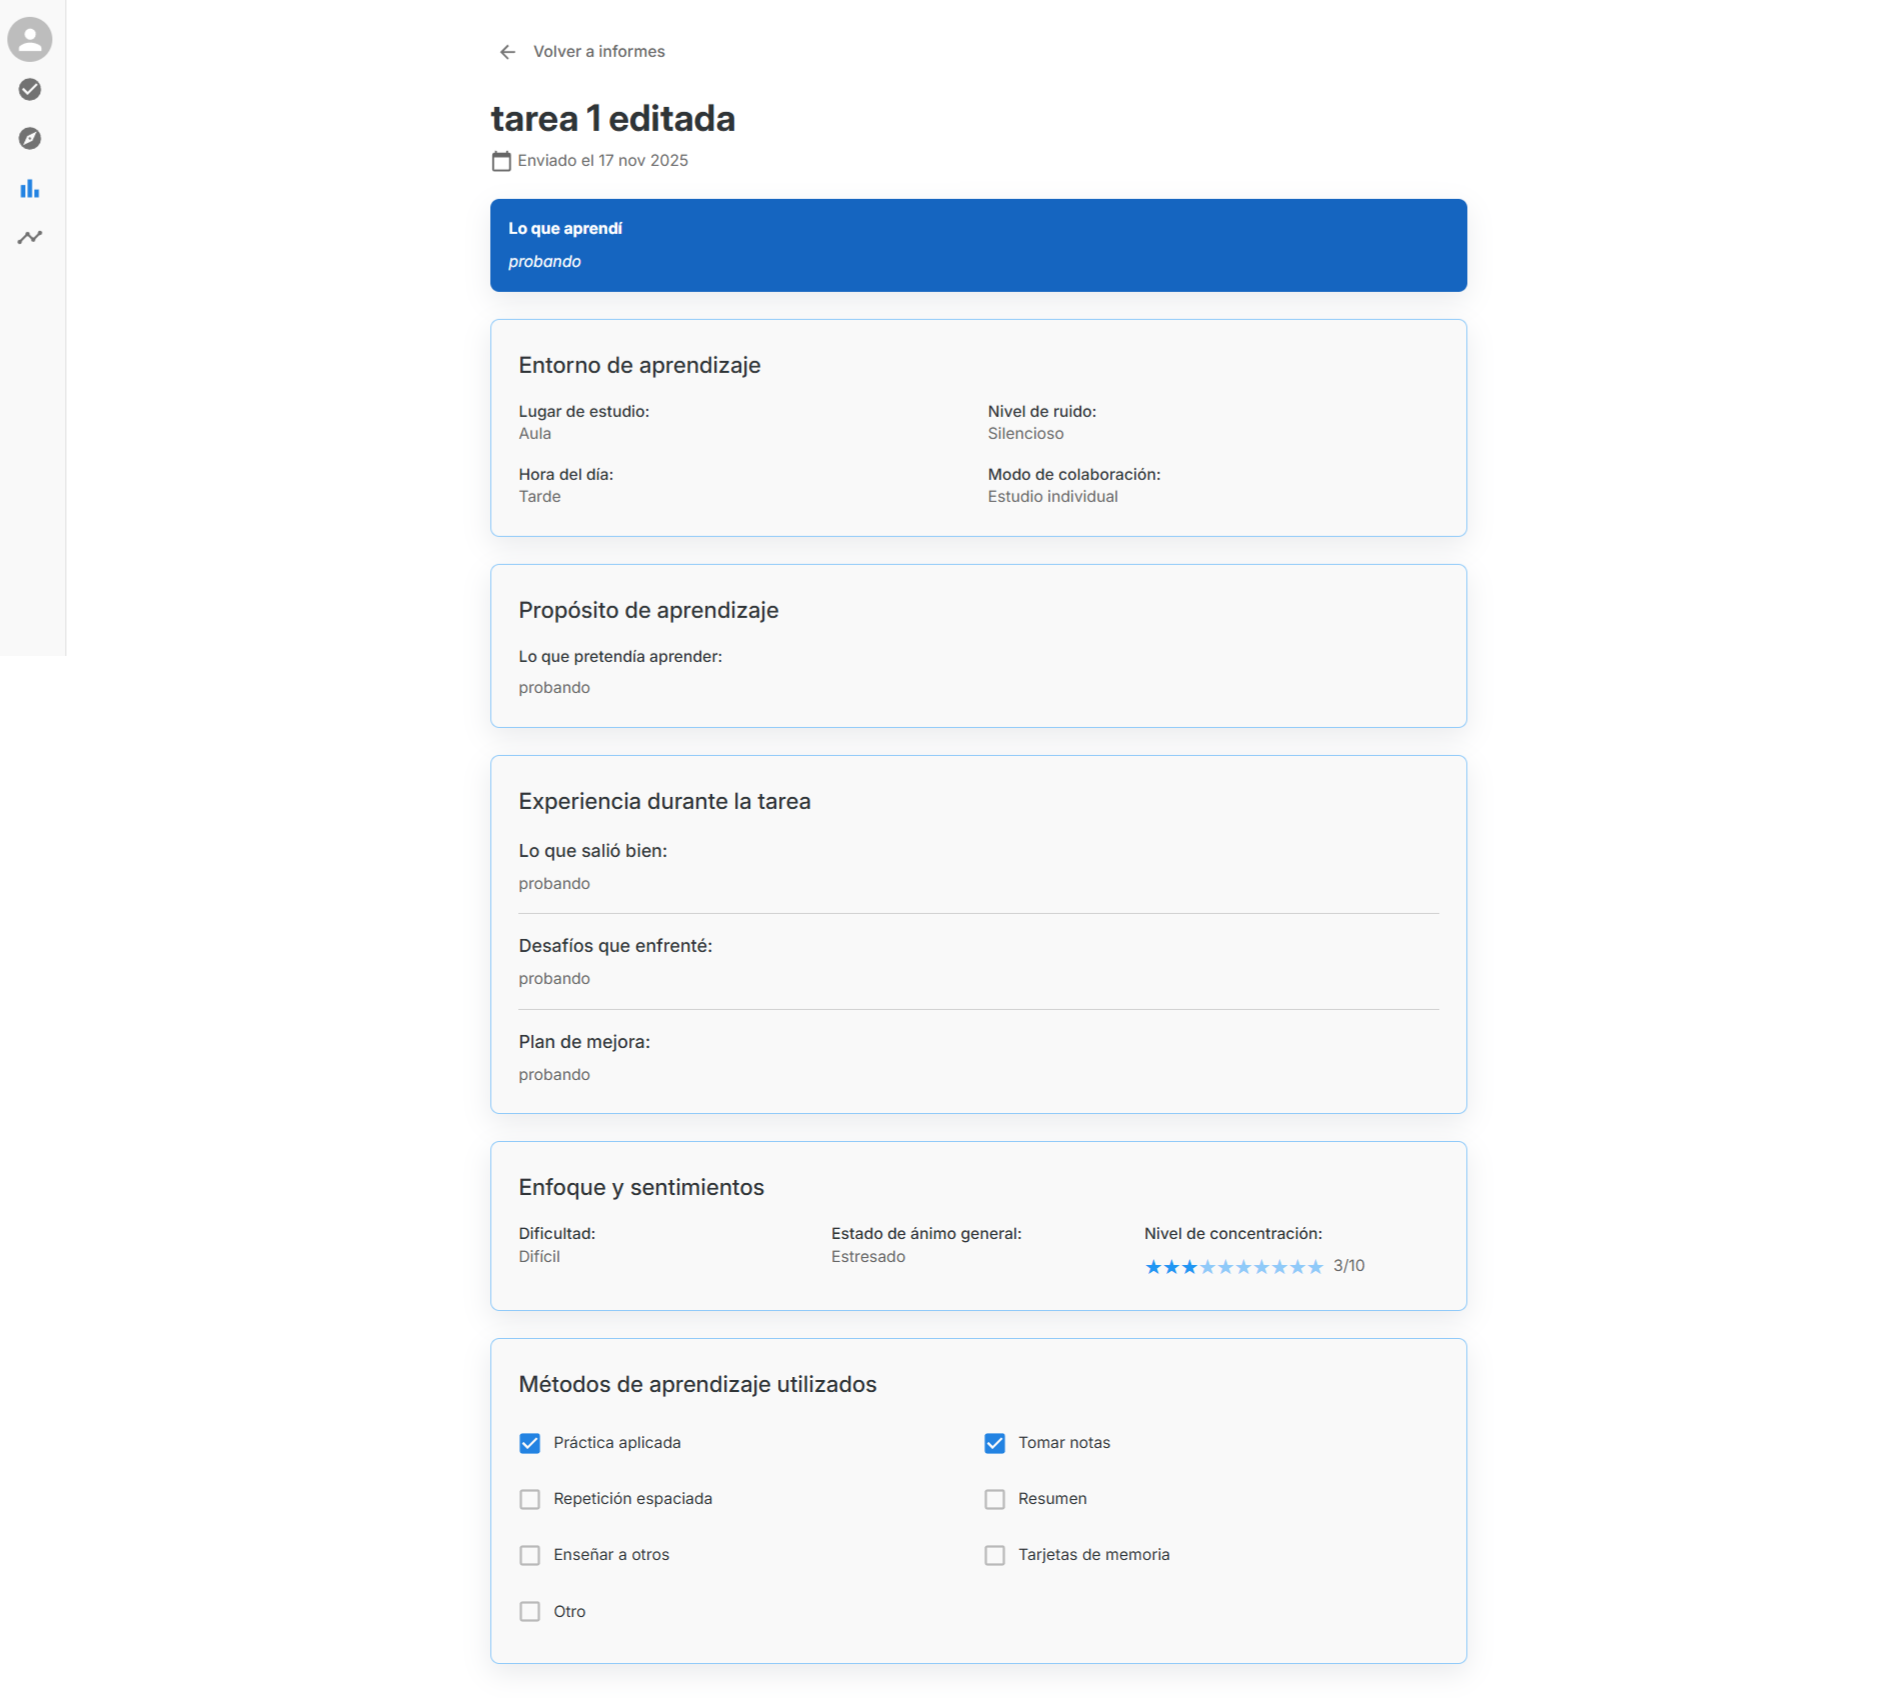
\includegraphics[width=0.95\textwidth]{Figuras/interfaces_AaA/reporte_detallado.png}
\caption{Vista detallada de un informe de aprendizaje asociado a una tarea completada.}
\label{fig:reporte-detallado}
\end{figure}

\noindent\textit{Descripción.} 
Cada informe consolida los datos registrados por el estudiante al finalizar la tarea. La vista incluye:  
(1) el entorno de estudio (lugar, nivel de ruido, colaboración y horario),  
(2) la intención de aprendizaje,  
(3) los aspectos logrados, desafíos encontrados y el plan de mejora,  
(4) indicadores complementarios como nivel de dificultad percibido, estado de ánimo y nivel de concentración,  
y (5) las estrategias de aprendizaje utilizadas.  

Esta estructura permite analizar la experiencia de estudio desde una perspectiva integral, facilitando el desarrollo de habilidades metacognitivas.

% -------------------------------------------------
\subsection*{Configuración de visibilidad de los planes de aprendizaje}
% -------------------------------------------------
% (1) Modal de configuración con visibilidad privada
\begin{figure}[H]
\centering
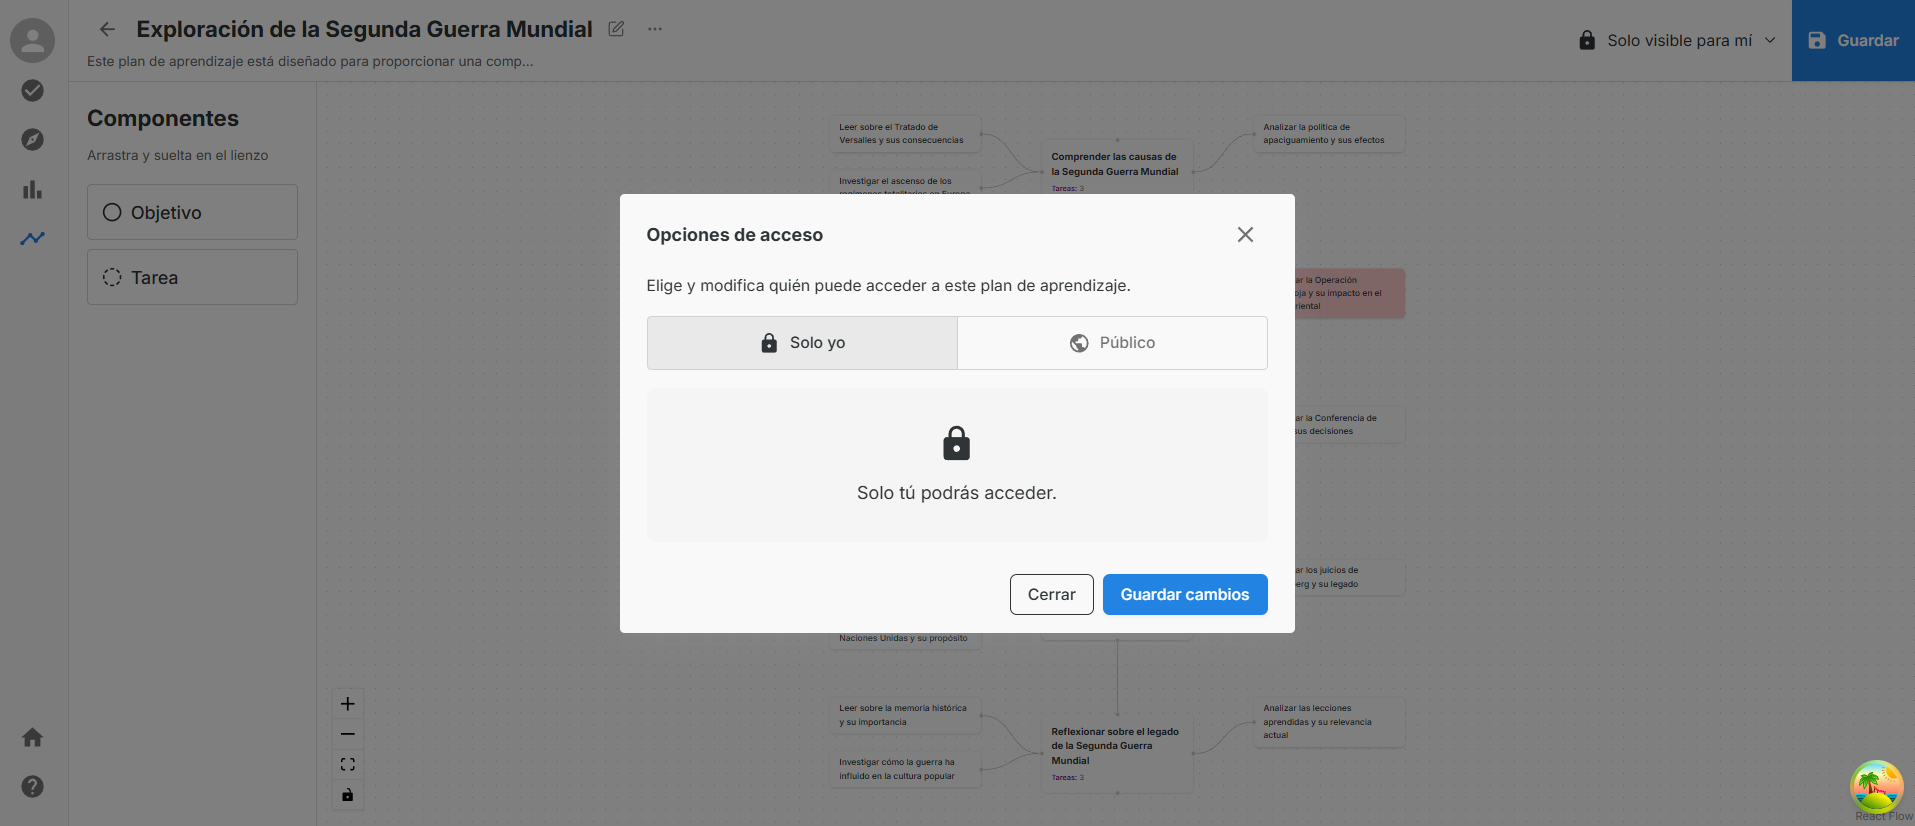
\includegraphics[width=0.95\textwidth]{Figuras/interfaces_AaA/visibilidad_privada.png}
\caption{Configuración de visibilidad de un plan de aprendizaje en modo privado.}
\label{fig:visibilidad-privada}
\end{figure}

\noindent\textit{Descripción.} En el modo \textit{Solo yo}, el plan permanece accesible únicamente para el estudiante, asegurando privacidad total durante su creación o revisión.

% (2) Modal de configuración con visibilidad pública mediante enlace
\begin{figure}[H]
\centering
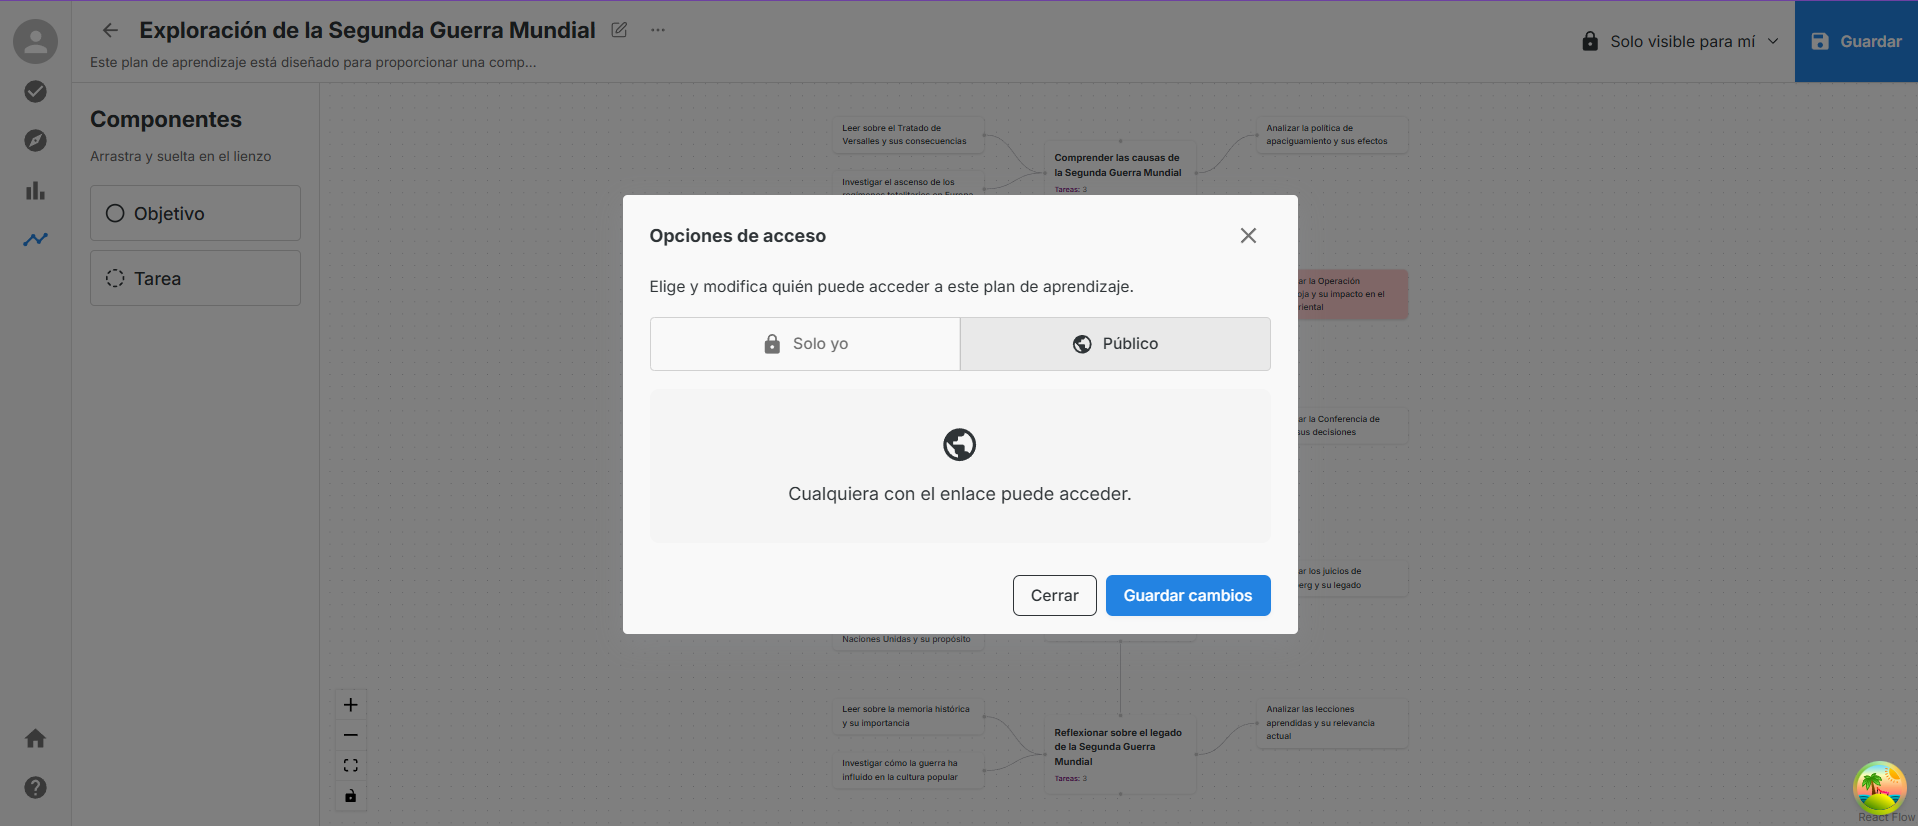
\includegraphics[width=0.95\textwidth]{Figuras/interfaces_AaA/visibilidad_publica.png}
\caption{Configuración de visibilidad que habilita el acceso público mediante enlace.}
\label{fig:visibilidad-publica-enlace}
\end{figure}

\noindent\textit{Descripción.} Al seleccionar la opción \textit{Público}, el sistema permite compartir el plan con cualquier persona que posea el enlace correspondiente, lo que facilita su difusión y reutilización en actividades colaborativas o procesos formativos.
